\documentclass[11pt,letterpaper]{article}

% --- Paquetes Principales ---
\usepackage[utf8]{inputenc}
\usepackage[spanish,es-nodecimaldot]{babel}
\usepackage[margin=2.5cm]{geometry}
\usepackage{amsmath,amssymb}
\usepackage{graphicx}
\usepackage{booktabs}
\usepackage{hyperref}
\usepackage{microtype}
\usepackage{xcolor}
\usepackage{caption}
\usepackage{subcaption}
\usepackage{float}
\usepackage[T1]{fontenc}
\usepackage{fancyhdr}
\setlength{\emergencystretch}{2em}

% --- Configuracion de Hipervinculos ---
\hypersetup{
    colorlinks=true,
    linkcolor=blue!70!black,
    citecolor=blue!70!black,
    urlcolor=blue!70!black
}

% --- Configuracion de Encabezados y Pies de Pagina (fancyhdr) ---
\pagestyle{fancy}
\fancyhf{}
\fancyhead[L]{\small\textsl{Boletín 02: Arboles de Búsqueda}}
\fancyhead[R]{\small\textsl{Bryan Aguirre F. --- Mat. 2024443402}}
\fancyfoot[C]{\thepage}
\renewcommand{\headrulewidth}{0.4pt}
\renewcommand{\footrulewidth}{0pt}

\begin{document}
\hypersetup{pageanchor=false}

\begin{titlepage}
    \centering
    
\includegraphics[width=0.42\textwidth]{logo_udec.png}\\[1.0cm]
    
    {\scshape\Large Universidad de Concepción \par}
    \vspace{0.25cm}
    {\scshape\large Facultad de Ingeniería \par}
    {\scshape\normalsize Departamento de Ingeniería Informática y Ciencias de la Computación \par}
    \vspace{1.2cm}
    
    {\Large\textbf{Estructuras de Datos y Algoritmos Avanzados (2026-2)}\par}
    \vspace{0.6cm}
    \rule{\linewidth}{0.6mm} \\[0.4cm]
    {\huge\bfseries Boletín 02: Arboles de Búsqueda \par}
    \vspace{0.3cm}
    {\large\textit{Análisis Teórico, Implementación en C++20 y Validación Experimental}\par}
    \rule{\linewidth}{0.6mm} \\[1.4cm]
    
    \begin{minipage}[t]{0.48\textwidth}
        \begin{flushleft} \large
            \textbf{Autor:}\\
            Bryan Eliseo Aguirre Fuentes\\[0.15cm]
            \textbf{Matrícula:}\\
            2024443402
        \end{flushleft}
    \end{minipage}
    \hfill
    \begin{minipage}[t]{0.48\textwidth}
        \begin{flushright} \large
            \textbf{Profesor:}\\
            Dr. José Fuentes\\[0.15cm]
            \textbf{Ayudante:}\\
            Leonardo Lovera
        \end{flushright}
    \end{minipage}
    
    \vfill
    {\large Concepción, Chile\\ \today \par}
\end{titlepage}
\hypersetup{pageanchor=true}


\pagenumbering{roman}
\pagestyle{plain}
\tableofcontents
\newpage

\pagenumbering{arabic}
\pagestyle{fancy}


\section{Resumen}
\subsection{Propósito y alcance del estudio}

En este trabajo se comparan tres implementaciones de árboles de búsqueda
compiladas en C++20: AVL, Rojo-Negro mediante \texttt{std::set} y Splay. Se
miden inserción, búsqueda y vaciado completo con claves únicas compartidas
entre árboles. Las consultas se generan tanto de manera uniforme como con
una binomial negativa que concentra accesos en claves populares.

En los ocho tamaños evaluados, el Rojo-Negro registra la menor media de
inserción y vaciado sin consultas previas, mientras que AVL registra la menor
media de búsqueda. Splay muestra la mayor mejora proporcional de búsqueda
cuando se concentran las consultas, aunque no alcanza el menor tiempo
absoluto. El patrón de búsquedas previas produce diferencias más pequeñas en
el vaciado posterior de Splay.


\subsection{Estructuras de Datos Analizadas}

A continuación una breve descripción de las estructuras de datos estudiadas:

\begin{itemize}
    \item \textbf{AVL}: El árbol AVL es un árbol binario de búsqueda que mantiene equilibradas las alturas de sus subárboles. Para cada nodo, la diferencia entre la altura izquierda y derecha se mantiene dentro de un rango acotado (A lo mas difieren en 1); si una inserción o eliminación rompe esa condición, el árbol se re equilibra mediante rotaciones
     \item \textbf{Red-Black Tree}: Un árbol Rojo-Negro es un árbol binario de búsqueda que mantiene el balance mediante colores y reglas sobre los nodos, esto con el fin de permitir más desbalanceo que un AVL tradicional, y así evitar computar muchas rotaciones en ambientes donde hay un alto flujo de inserciones. Después de insertar o eliminar claves, aplica recoloreos y rotaciones para conservar esas reglas y mantener la altura proporcional a \(\log n\).
      \item \textbf{Splay Tree}: El Splay es un árbol binario de búsqueda autoajustable. Después de acceder a una clave, la lleva a la raíz mediante rotaciones, que pueden ser de tipo zig, zig-zig o zig-zag. Este reajuste tiene como fin favorecer claves consultadas con frecuencia, pero modifica la estructura durante la búsqueda.
\end{itemize}


\newpage

\section{Análisis Teórico}

En esta sección se analizan las complejidades temporales y espaciales de las estructuras estudiadas. Para cada operación se presentan sus cotas asintóticas, distinguiendo el peor caso individual, además se describen los requerimientos de memoria de cada estructura.

\subsection{AVL}

\begin{itemize}
    \item \textbf{Insert:} La inserción sigue inicialmente el orden de un árbol
    binario de búsqueda. Luego se actualizan las alturas o factores de balance
    en los nodos del camino recorrido y se aplican rotaciones cuando es
    necesario. Como la altura de un AVL es $O(\log n)$, el tiempo de inserción
    en el peor caso es $O(\log n)$ .

    \item \textbf{Search:} La búsqueda compara la clave con los nodos desde la
    raíz y continúa por el subárbol correspondiente. Debido a que la altura del
    árbol está acotada por $O(\log n)$, su tiempo en el peor caso es
    $O(\log n)$.

    \item \textbf{Delete:} Primero se busca el nodo que se eliminará y se
    realiza la eliminación como en un árbol binario de búsqueda. Después se
    actualiza el balance en el camino hacia la raíz y pueden aplicarse
    rotaciones en varios niveles. Tanto la búsqueda como el rebalanceo toman
    $O(\log n)$ en el peor caso.

    \item \textbf{Espacio en memoria:} La estructura requiere $O(n)$ espacio
    para almacenar sus $n$ nodos. Cada nodo guarda la clave, enlaces a sus hijos
    y un dato auxiliar constante, como su altura o factor de balance. Una
    implementación recursiva utiliza además una pila de llamadas de
    $O(\log n)$, dado que la altura del AVL es logarítmica.
\end{itemize}

\subsection{Red-Black Tree}

En análisis teórico será basado en la implementación usando el método std::set de la biblioteca estándar de C++.

\begin{itemize}
    \item \textbf{Insert:} La inserción por clave se realiza con
    \texttt{std::set::insert}. El estándar establece complejidad logarítmica $O(\log n)$
    para esta operación; en libstdc++, \texttt{std::set} se implementa sobre un
    árbol Rojo-Negro.

    \item \textbf{Search:} La búsqueda se realiza con \texttt{std::set::find}.
    La operación tiene complejidad $O(\log n)$ en el peor caso para los contenedores asociativos ordenados.

    \item \textbf{Delete:} La eliminación por clave se realiza con
    \texttt{std::set::erase(key)} y tiene complejidad $O(\log n)$. La estructura puede recolorear nodos y aplicar
    rotaciones para conservar las propiedades del árbol Rojo-Negro.

    \item \textbf{Espacio en memoria:} El contenedor necesita $O(n)$ espacio
    para sus nodos. Cada nodo almacena la clave, enlaces y la información de
    color; el tamaño exacto en bytes depende de la implementación, los
    punteros, la alineación y el asignador de memoria.
\end{itemize}

\subsection{Splay Tree}
\begin{itemize}
    \item \textbf{Insert:} La inserción busca la posición de la clave y luego
    realiza operaciones de splaying para reorganizar el árbol. Su costo
    amortizado es $O(\log n)$ por operación sobre una secuencia de operaciones;
    una operación individual puede tomar $O(n)$ en el peor caso.

    \item \textbf{Search:} La búsqueda puede reorganizar el árbol y acercar la
    clave accedida a la raíz mediante rotaciones. Su costo amortizado es
    $O(\log n)$, aunque una búsqueda individual puede tomar $O(n)$ en el peor
    caso.

    \item \textbf{Delete:} La eliminación localiza y splayea la clave antes de
    retirarla y unir los subárboles resultantes. Su costo amortizado es
    $O(\log n)$ por operación; el peor caso individual es $O(n)$.

    \item \textbf{Espacio en memoria:} La estructura necesita $O(n)$ espacio
    para almacenar sus nodos. Cada nodo guarda la clave y enlaces a sus hijos;
    según la implementación, también puede guardar un enlace al padre. No
    requiere almacenar alturas o colores para mantener el balance. Como el
    Splay puede alcanzar altura $O(n)$, una implementación recursiva puede
    necesitar una pila de llamadas de $O(n)$ en el peor caso.

    \textbf{Nota:} Al no mantener una restricción de balanceo, si insertamos claves en un orden particular, como en orden creciente, podemos degradar la estructura a una lista enlazada, volviendo $O(n)$ el tiempo en el peor caso.
\end{itemize}

\begin{table}[ht]
    \centering
    \caption{Complejidad temporal en el peor caso de las operaciones}
    \label{tab:complejidad-arboles}
    \begin{tabular}{|l|c|c|c|}
        \hline
        \textbf{Estructura} & \textbf{Insertar} & \textbf{Buscar} & \textbf{Eliminar} \\
        \hline
        Árbol AVL & $O(\log n)$ & $O(\log n)$ & $O(\log n)$ \\
        \hline
        Rojo-Negro mediante \texttt{std::set} & $O(\log n)$ & $O(\log n)$ & $O(\log n)$ \\
        \hline
        Splay Tree & $O(n)$ & $O(n)$ & $O(n)$ \\
        \hline
    \end{tabular}
\end{table}

\noindent
En el árbol AVL, la altura se mantiene en $O(\log n)$, por lo que las tres
operaciones tienen esa cota en el peor caso. Para el árbol Rojo-Negro se usa
\texttt{std::set}; la tabla describe la complejidad de insertar, buscar con
\texttt{find} y eliminar por clave con \texttt{erase(clave)}. En un Splay Tree,
una operación individual puede tomar $O(n)$ en el peor caso, aunque el costo
amortizado de las operaciones es $O(\log n)$.

\textbf{Nota}: El uso de memoria es lineal $\mathcal{O}(n)$ en las tres estructuras, ya que almacenan $n$ elementos, aunque AVL y Red-Black requieren unos bits extra por nodo para mantener colores o factores de balanceo.



\newpage

\section{Implementaciones}

Las implementaciones de todos los arboles de búsqueda fueron obtenidas y adaptadas de diferentes repositorios, están implementadas en C++ 20, compiladas bajo
el estándar industrial con el compilador g++ y optimizaciones de nivel -O3 -march=native.

El código fuente completo se encuentra modularizado en archivos de encabezado dentro del directorio \texttt{include/} y se adjunta de manera íntegra en el archivo comprimido (\texttt{.zip}) que acompaña a este informe. Asimismo, para replicar los experimentos, acceder a los scripts de automatización del banco de pruebas o consultar las implementaciones, se encuentra disponible el repositorio público del proyecto:

\begin{center}
\href{https://github.com/StackDs/EDAA-Experiments}{ Repositorio}
\end{center}

Las estructuras se organizan en los encabezados de \texttt{include/trees/}
como clases plantilla parametrizadas por el tipo de clave \texttt{Key} y
el comparador \texttt{Compare}, cuyo valor predeterminado es
\texttt{std::less<Key>}. Todas almacenan claves únicas: dos claves son
equivalentes si ninguna precede a la otra según el comparador. Comparten
las operaciones \texttt{insert}, \texttt{search} y \texttt{erase}, que
retornan un booleano para indicar si se insertó, encontró o eliminó una
clave, respectivamente, además de \texttt{size} y \texttt{empty}.

\subsection{Árbol AVL}

La clase \texttt{AVLTree}, definida en \texttt{avl\_tree.h}, adapta la
organización recursiva y los casos de rebalanceo de \textit{AVLTree},
según la atribución del encabezado.

\begin{itemize}
    \item \textbf{Nodos y propiedad de la memoria:}
    Cada nodo almacena una clave, una altura y dos hijos mediante
    \texttt{std::unique\_ptr<Node>}. La raíz también utiliza este tipo
    de puntero, por lo que cada nodo tiene un único propietario y su
    memoria se libera automáticamente al eliminarlo o destruir el árbol.
    Los punteros obtenidos con \texttt{get()} permiten recorrer los nodos
    sin adquirir su propiedad. No se almacena un puntero al padre: la
    recursión conserva el camino de regreso hacia la raíz.

    \item \textbf{Equilibrio y rotaciones:}
    Se considera altura cero para un enlace nulo y uno para una hoja.
    Tras modificar un subárbol se recalcula su altura y el factor
    $b=h_{\mathrm{izq}}-h_{\mathrm{der}}$. Si $|b|>1$, se aplican
    rotaciones simples (LL o RR) o dobles (LR o RL).
    Los enlaces se transfieren mediante \texttt{std::move}, sin copiar
    nodos. Por ejemplo, una rotación derecha eleva al hijo izquierdo,
    conecta su antiguo hijo derecho como hijo izquierdo del nodo original
    y deja este último a la derecha de la nueva raíz. Las funciones
    reciben el enlace propietario por referencia para poder sustituir
    la raíz del subárbol y actualizar las alturas afectadas.

    \item \textbf{Operaciones:}
    La inserción crea una hoja con \texttt{std::make\_unique} tras
    descender recursivamente; si la clave ya existe, no la duplica.
    La búsqueda es iterativa y no modifica el árbol. Para eliminar un
    nodo con cero o un hijo se sustituye su enlace por el hijo restante,
    que puede ser nulo. Si tiene dos hijos, se copia la clave del mínimo
    del subárbol derecho y luego se elimina ese sucesor. Al regresar de
    la recursión se restablece el equilibrio. El contador de elementos
    cambia una sola vez por inserción o eliminación exitosa.
\end{itemize}

\subsection{Árbol Splay}

En \texttt{splay\_tree.h} se define la clase \texttt{SplayTree}, que
adapta las rotaciones ascendentes de \textit{Boost.Intrusive}, según
la atribución del encabezado.

\begin{itemize}
    \item \textbf{Nodos y manejo de punteros:}
    Cada nodo contiene una clave y tres punteros \texttt{Node*}:
    \texttt{left}, \texttt{right} y \texttt{parent}. El árbol administra
    su memoria con \texttt{new} y \texttt{delete}; el enlace al padre
    sirve para ascender y no implica propiedad adicional. Las rotaciones
    reconectan los hijos, sus padres y el enlace desde el abuelo; también
    actualizan \texttt{root\_} cuando cambia la raíz, cuyo padre queda
    en \texttt{nullptr}.

    \item \textbf{Ajuste mediante \texttt{splay}:}
    El nodo accedido asciende hasta la raíz mediante tres casos:
    \textit{Zig}, una rotación cuando su padre es la raíz;
    \textit{Zig--Zig}, dos rotaciones en la misma dirección cuando
    nodo y padre están alineados; y \textit{Zig--Zag}, dos rotaciones
    opuestas cuando están cruzados. El proceso es iterativo y conserva
    el orden de búsqueda, sin almacenar alturas ni colores.

    \item \textbf{Operaciones y liberación:}
    La inserción enlaza una nueva hoja y la lleva a la raíz; si la clave
    existe, lleva a la raíz el nodo encontrado. La búsqueda hace lo
    mismo cuando tiene éxito y, si falla, ajusta el último nodo visitado.
    Por ello, \texttt{search} puede modificar el árbol incluso al
    retornar \texttt{false}. Para eliminar una clave presente, primero
    se la lleva a la raíz y se libera ese nodo. Si hay subárbol izquierdo,
    su máximo se lleva a la raíz y recibe como hijo derecho el subárbol
    derecho original, actualizando los enlaces al padre; en caso
    contrario, el subárbol derecho pasa a ser la raíz. Una eliminación
    fallida también ajusta el último nodo visitado. El destructor ejecuta
    \texttt{clear}, que alterna rotaciones derechas y eliminación de
    raíces sin hijo izquierdo, evitando una limpieza recursiva sobre
    árboles degenerados. La copia y el movimiento de la clase están
    deshabilitados para evitar compartir accidentalmente sus nodos.
\end{itemize}

\subsection{Árbol Rojo-Negro mediante la STL}

La clase \texttt{RedBlackTree}, definida en \texttt{red\_black\_tree.h},
es un adaptador propio del contenedor \texttt{std::set}, parametrizado
por \texttt{Key} y \texttt{Compare}.

\begin{itemize}
    \item \textbf{Representación y memoria:}
    En \texttt{libstdc++}, el contenedor utiliza un árbol rojo-negro cuyos
    nodos almacenan la clave, el color y enlaces al padre y a los hijos.
    La biblioteca administra la reserva y liberación de memoria, así como
    las rotaciones y recoloreos que mantienen el equilibrio. El adaptador
    no manipula estos nodos directamente. Esta representación depende de
    la biblioteca: el estándar de C++ no exige que \texttt{std::set} se
    implemente con un árbol rojo-negro.

    \item \textbf{Interfaz común:}
    La inserción devuelve el indicador de \texttt{values\_.insert}; la
    búsqueda comprueba si \texttt{find} retorna un iterador distinto de
    \texttt{end}; y la eliminación verifica si \texttt{erase} suprimió
    algún elemento. Tanto \texttt{size} como \texttt{empty} se delegan
    al contenedor. Así se dispone de una referencia de biblioteca con la
    misma interfaz de operaciones que las otras estructuras.
\end{itemize}
\newpage

\section{Diseño y Resultados Experimentales}

\subsection{Decisiones de Inicialización y Datasets}

No se utilizaron conjuntos de datos externos. Para cada tamaño
\[
n\in\{1\,000,2\,000,4\,000,8\,000,16\,000,32\,000,64\,000,128\,000\}
\]
se generan las claves únicas $1,\ldots,n$ y se barajan con
\texttt{std::shuffle}. La semilla depende únicamente de $n$ y de la
repetición; por ello, las tres implementaciones reciben el mismo orden de
inserción. Los órdenes de eliminación también coinciden entre árboles para
una misma repetición. Las claves son enteros de 64 bits.

Para estudiar las búsquedas se preparan dos secuencias de consultas exitosas:
\begin{itemize}
    \item \textbf{Uniforme:} cada clave presente se selecciona con la misma
    probabilidad.
    \item \textbf{Binomial negativa:} se barajan las claves para asignarles
    rangos de popularidad $0,\ldots,n-1$. Se sortea un rango
    $R\sim\operatorname{NB}(2,p)$, con
    $p=3/(0{,}05n+3)$, y se vuelve a sortear cuando $R\geq n$.
    Aproximadamente el 80\% de las consultas se concentra en el primer 5\%
    de los rangos. La asignación aleatoria evita asociar popularidad con
    claves numéricamente pequeñas.
\end{itemize}

Cada repetición de búsqueda ejecuta $5n$ consultas de preparación fuera del
reloj y cronometra otras $10n$. En el escenario de eliminación D1 se ejecutan
ambas tandas, $15n$ consultas, \emph{antes} de cronometrar el vaciado. La
distribución de D1 describe, por tanto, las búsquedas previas y no el orden de
eliminación. D0 vacía el árbol sin consultas previas. Los tres árboles se
comparan en D0; D1 se estudia solo en Splay porque sus búsquedas reorganizan
la estructura.

La batería automatizada configura 64 repeticiones por tamaño, afinidad al
núcleo lógico 2 con \texttt{taskset} y una pausa de dos segundos entre series.
Se compila con \texttt{g++} en C++20 y las opciones
\texttt{-O3 -march=native}. La generación de claves y consultas, la población
previa del árbol y la preparación quedan fuera del intervalo medido. Se
cronometra el lote completo y se divide su duración por $n$ inserciones,
$10n$ búsquedas o $n$ eliminaciones, según la fase. Los archivos CSV contienen
la media, la desviación estándar muestral y cinco cuantiles de los tiempos
por operación. Las barras de las figuras representan una desviación estándar,
no intervalos de confianza; su extremo inferior se limita a cero.

\subsection{Características de la Máquina}
Los experimentos se ejecutaron sobre una estación de trabajo con las siguientes especificaciones:
\begin{itemize}
    \item \textbf{Procesador (CPU):} 13th Gen Intel(R) Core(TM) i5-13420H (Arquitectura Raptor Lake, 8 núcleos / 12 hilos: 4 P-Cores + 4 E-Cores), frecuencia base 2.10 GHz y Turbo máxima 4.60 GHz. Jerarquía de cachés: L1d de 320 KiB, L1i de 384 KiB, L2 de 7 MiB y L3 compartida de 12 MiB Intel Smart Cache.
    \item \textbf{Memoria Principal (RAM):} 16 GiB DDR (15 GiB utilizables en sistema operativo).
    \item \textbf{Memoria Secundaria (Almacenamiento):} Unidad de estado sólido (SSD) NVMe WD PC SN740 de 512 GB (interfaz PCIe Gen4 $\times$4).
    \item \textbf{Entorno de compilación:} Sistema operativo Arch Linux x86\_64 (Kernel 6.x), compilador GCC con banderas \texttt{-std=c++20 -O3 -march=native}.
    \item \textbf{Afinidad y Aislamiento de CPU (Asignación a P-Core):} 
    Dado que el procesador cuenta con una arquitectura híbrida de núcleos P y E, el proceso de medición fue anclado mediante afinidad de CPU (\texttt{taskset -c 2}) a un núcleo lógico. Esto reduce las variaciones debidas a migraciones del proceso, pero no elimina las fluctuaciones de frecuencia, temperatura o actividad del sistema.
\end{itemize}

\subsection{Resultados Experimentales}

Los resultados siguientes proceden de los 14 CSV de \texttt{data/}. Todas las
figuras presentan el tamaño inicial $n$ en escala logarítmica y el tiempo
medio por operación en nanosegundos. Una curva menor indica menos tiempo
para el lote medido, una vez normalizado por el número de operaciones. La
Tabla~\ref{tab:resumen128k} reúne un punto de referencia numérico del tamaño
máximo; las figuras muestran los ocho tamaños.

\begin{table}[htbp]
    \centering
    \caption{Tiempo medio $\pm$ desviación estándar en ns por operación para
    $n=128\,000$. El guion indica un escenario no ejecutado.}
    \label{tab:resumen128k}
    \small
    \begin{tabular}{lccc}
        \toprule
        \textbf{Operación y escenario} & \textbf{AVL} & \textbf{Rojo-Negro} & \textbf{Splay} \\
        \midrule
        Inserción & $848\pm65$ & $470\pm43$ & $1\,048\pm66$ \\
        Búsqueda uniforme & $606\pm36$ & $724\pm22$ & $1\,352\pm29$ \\
        Búsqueda binomial negativa & $509\pm18$ & $611\pm16$ & $661\pm22$ \\
        Vaciado D0 & $814\pm69$ & $778\pm64$ & $1\,439\pm97$ \\
        Vaciado D1 tras uniforme & --- & --- & $1\,499\pm93$ \\
        Vaciado D1 tras binomial negativa & --- & --- & $1\,456\pm90$ \\
        \bottomrule
    \end{tabular}
\end{table}

\subsubsection{Experimento 1: Inserción variando el tamaño ($n$)}

Se inserta la misma permutación de claves en un árbol inicialmente vacío.
La Figura~\ref{fig:b02-insercion} compara el tiempo medio por inserción de
las tres implementaciones. La construcción del vector y su barajado no forman
parte del tiempo representado.

\paragraph{Hipótesis.}
Se espera un aumento moderado del costo por inserción al crecer $n$, en
consonancia con las cotas logarítmicas de AVL y Rojo-Negro y la cota
amortizada logarítmica de Splay. Se plantea que el adaptador de
\texttt{std::set} obtenga tiempos bajos por la implementación de biblioteca,
mientras que las rotaciones de Splay agreguen trabajo a esta operación.1

\begin{figure}[H]
    \centering
    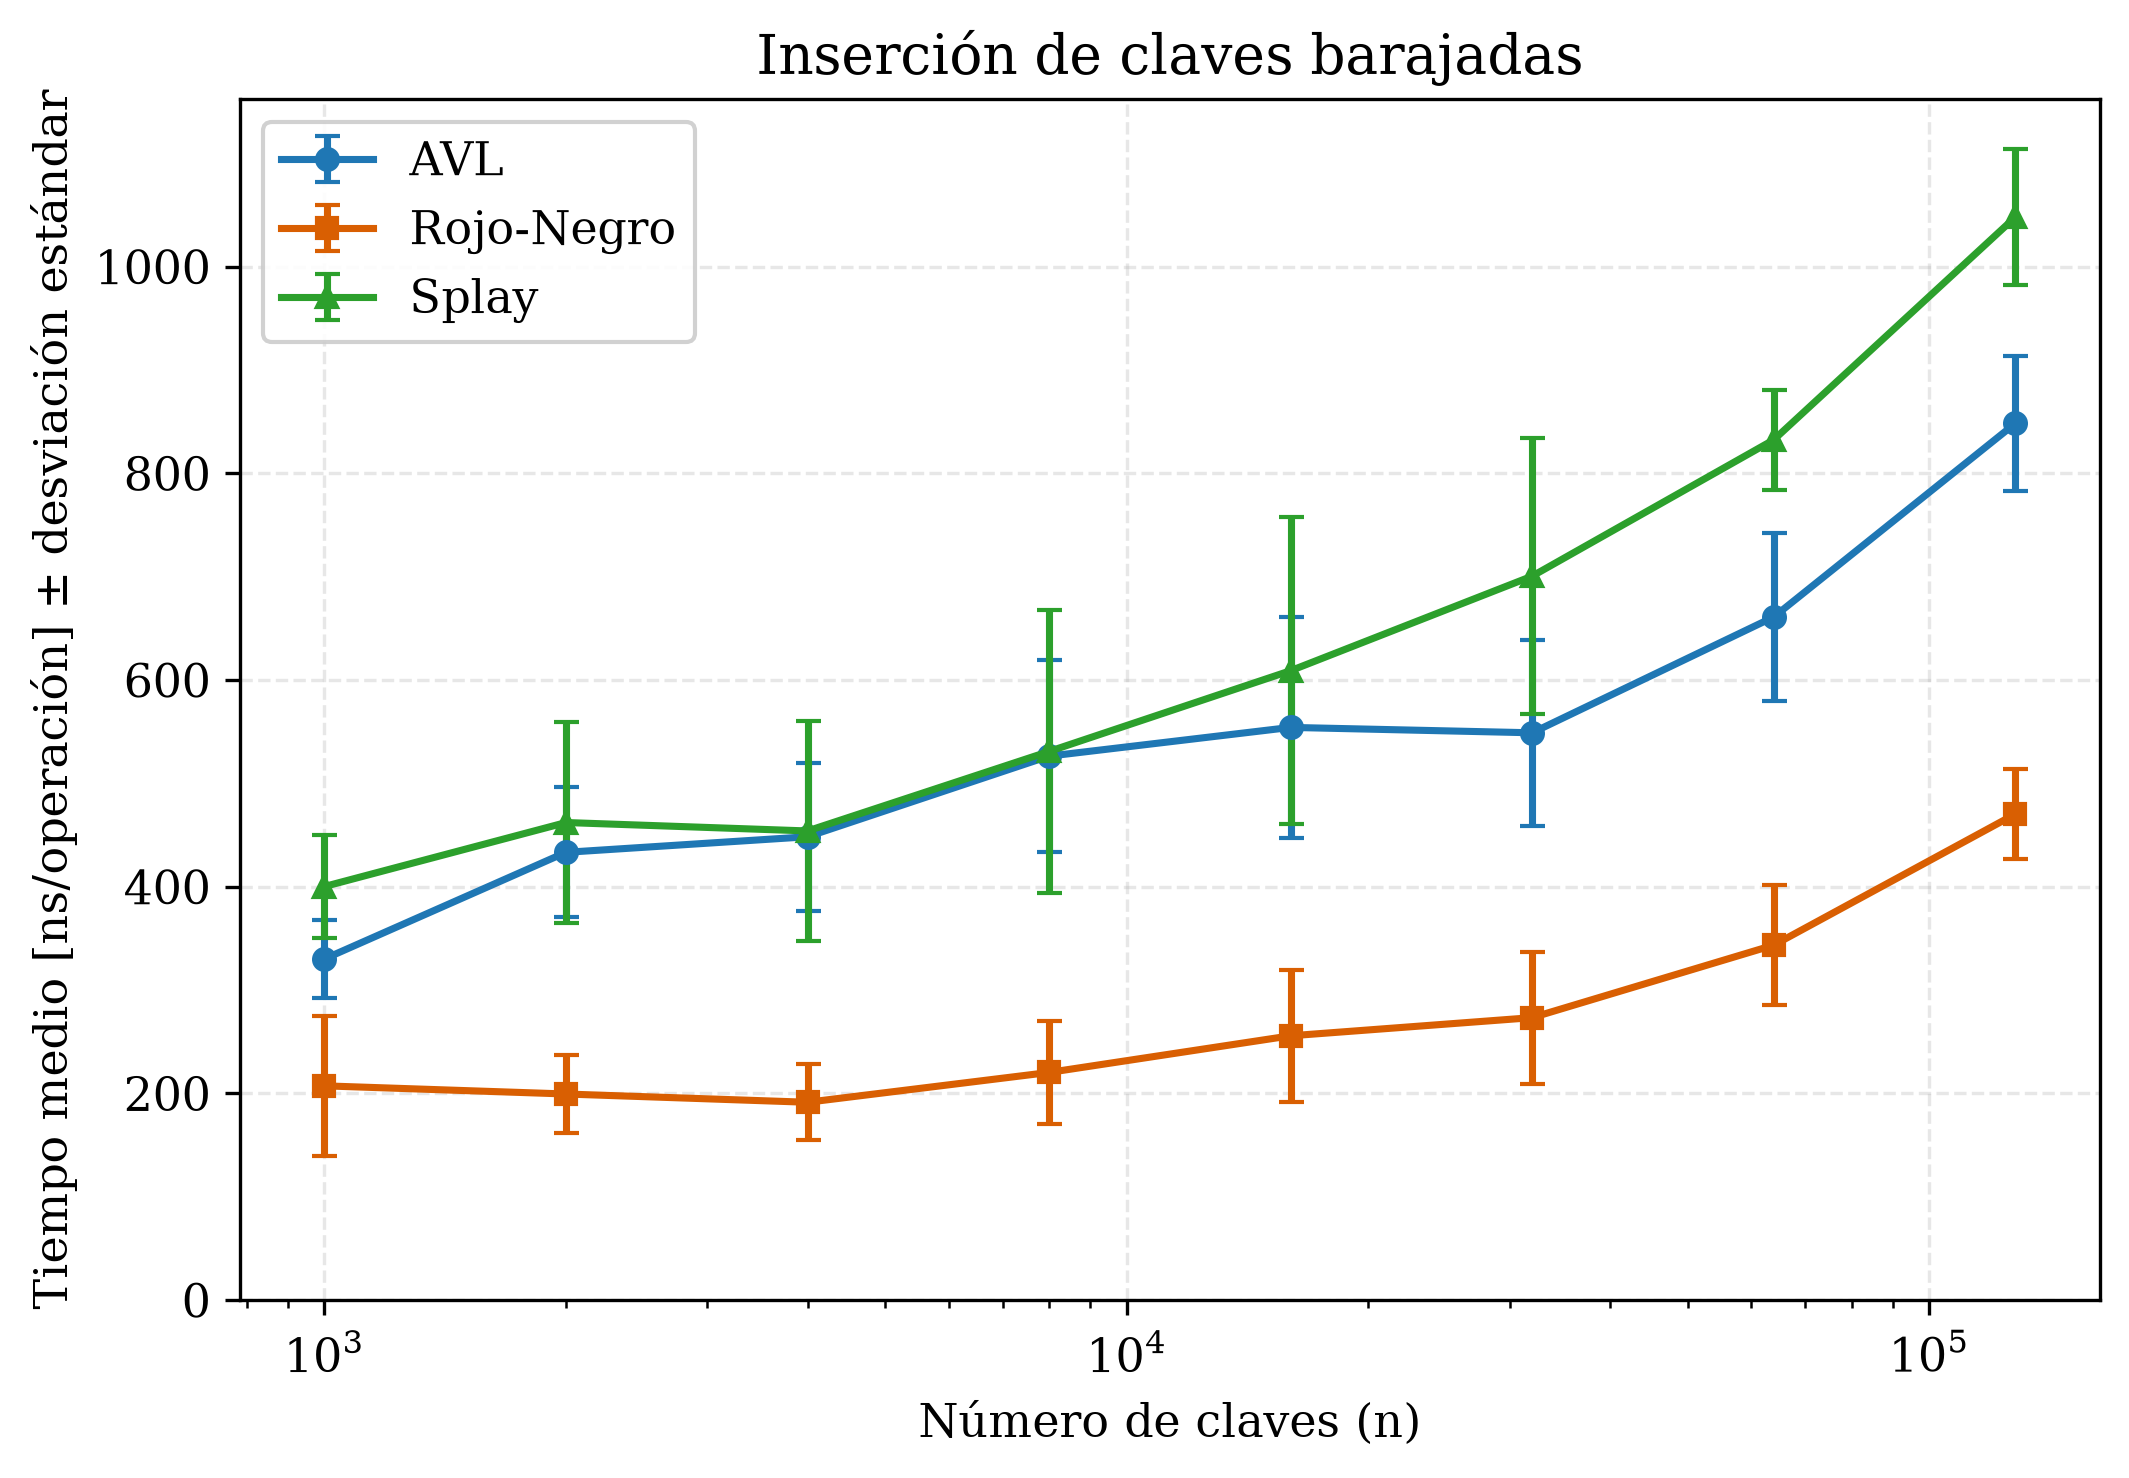
\includegraphics[width=0.84\textwidth]{../plots/por_tamano/fig_insercion_general_sin_especificar.png}
    \caption{Inserción: comparación de AVL, Rojo-Negro y Splay sobre las
    mismas claves barajadas. Cada punto es el tiempo del lote dividido por
    $n$; las barras indican una desviación estándar.}
    \label{fig:b02-insercion}
\end{figure}

\paragraph{Observaciones.}
El Rojo-Negro registra el menor tiempo medio en los ocho tamaños. En
$n=128\,000$ alcanza $470$ ns por inserción, frente a $848$ ns de AVL y
$1\,048$ ns de Splay. Los tres tiempos por operación aumentan con el tamaño:
entre $n=1\,000$ y $n=128\,000$, las medias pasan de $207$ a $470$ ns en
Rojo-Negro, de $330$ a $848$ ns en AVL y de $400$ a $1\,048$ ns en Splay.
Este patrón es compatible con un costo creciente, pero el intervalo de
tamaños y estas mediciones no bastan para estimar una cota asintótica.

\subsubsection{Experimento 2: Búsqueda uniforme y binomial negativa}

Con los árboles ya poblados, se comparan búsquedas exitosas uniformes con
consultas concentradas mediante binomial negativa. Las
Figuras~\ref{fig:b02-busqueda-uniforme} y~\ref{fig:b02-busqueda-binomial}
muestran, por separado, los tres árboles bajo cada carga. Las
Figuras~\ref{fig:b02-dist-avl}, \ref{fig:b02-dist-rb}
y~\ref{fig:b02-dist-splay} fijan el árbol y superponen sus dos cargas; estas
últimas son gráficos de \emph{tiempo de búsqueda}, no histogramas de
frecuencia de claves.

\paragraph{Hipótesis.}
Se espera que Splay obtenga la mayor reducción proporcional al repetir
consultas sobre un subconjunto pequeño: los accesos llevan esas claves hacia
la raíz. AVL y Rojo-Negro no se reorganizan al buscar, aunque sus tiempos
también pueden cambiar por la profundidad de las claves seleccionadas y la
localidad de memoria. La hipótesis no presupone que Splay sea el más rápido
en valor absoluto.

\begin{figure}[H]
    \centering
    \begin{subfigure}[t]{0.48\textwidth}
        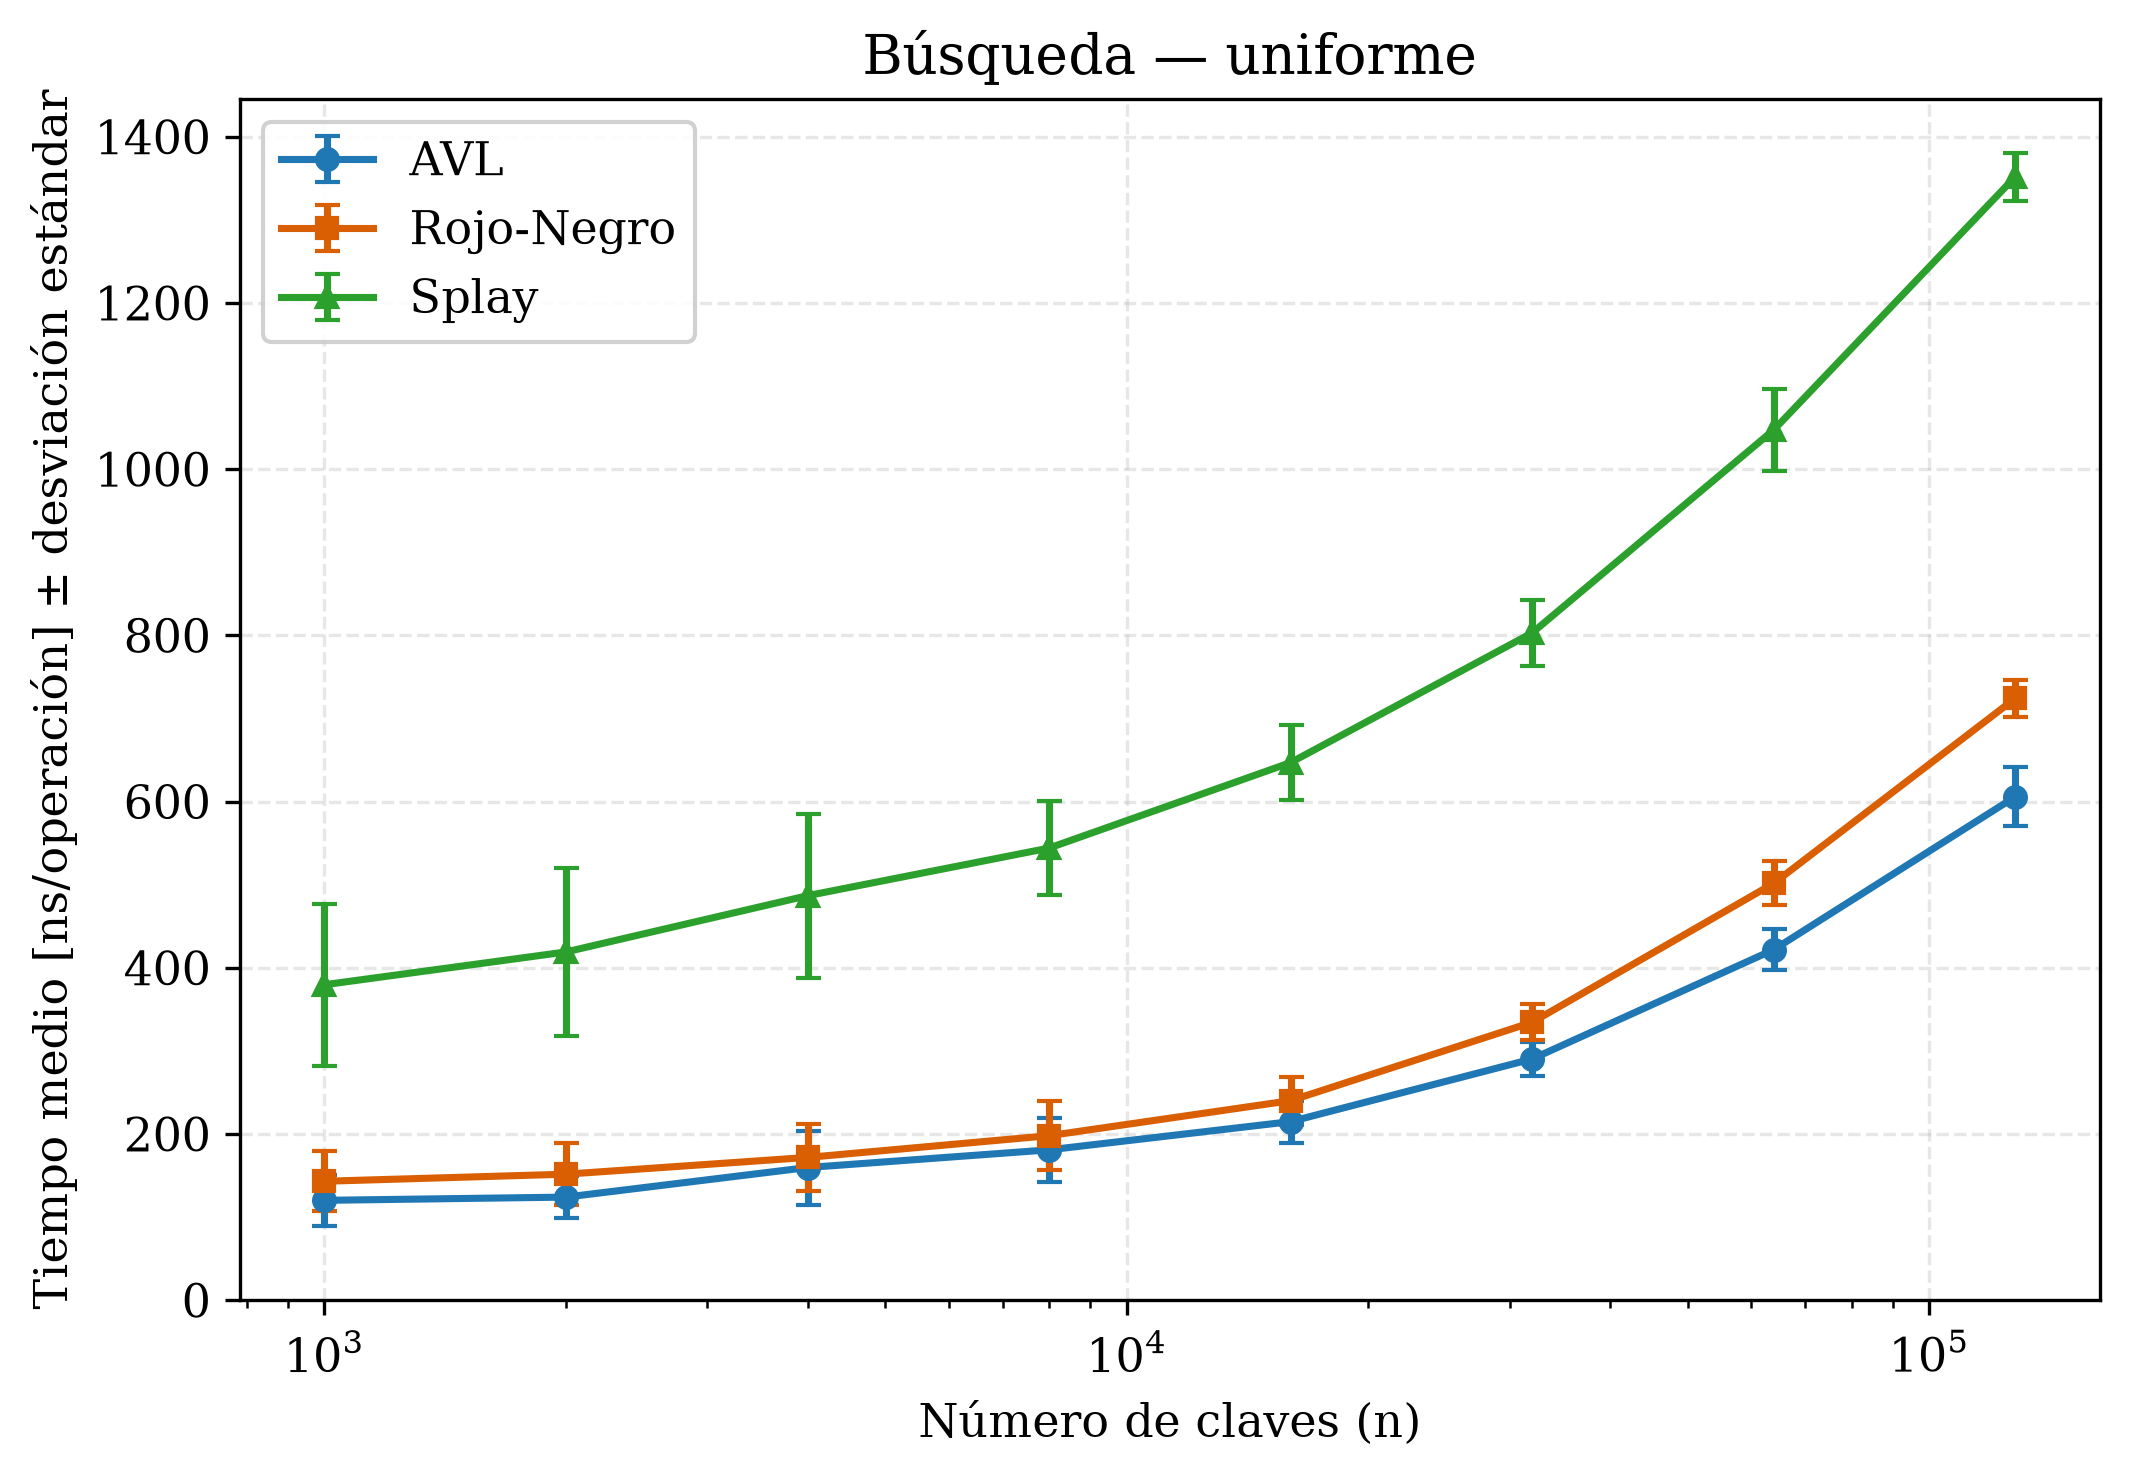
\includegraphics[width=\textwidth]{../plots/por_tamano/fig_busqueda_general_uniforme.png}
        \caption{Consultas uniformes: cada clave tiene igual probabilidad.}
        \label{fig:b02-busqueda-uniforme}
    \end{subfigure}
    \hfill
    \begin{subfigure}[t]{0.48\textwidth}
        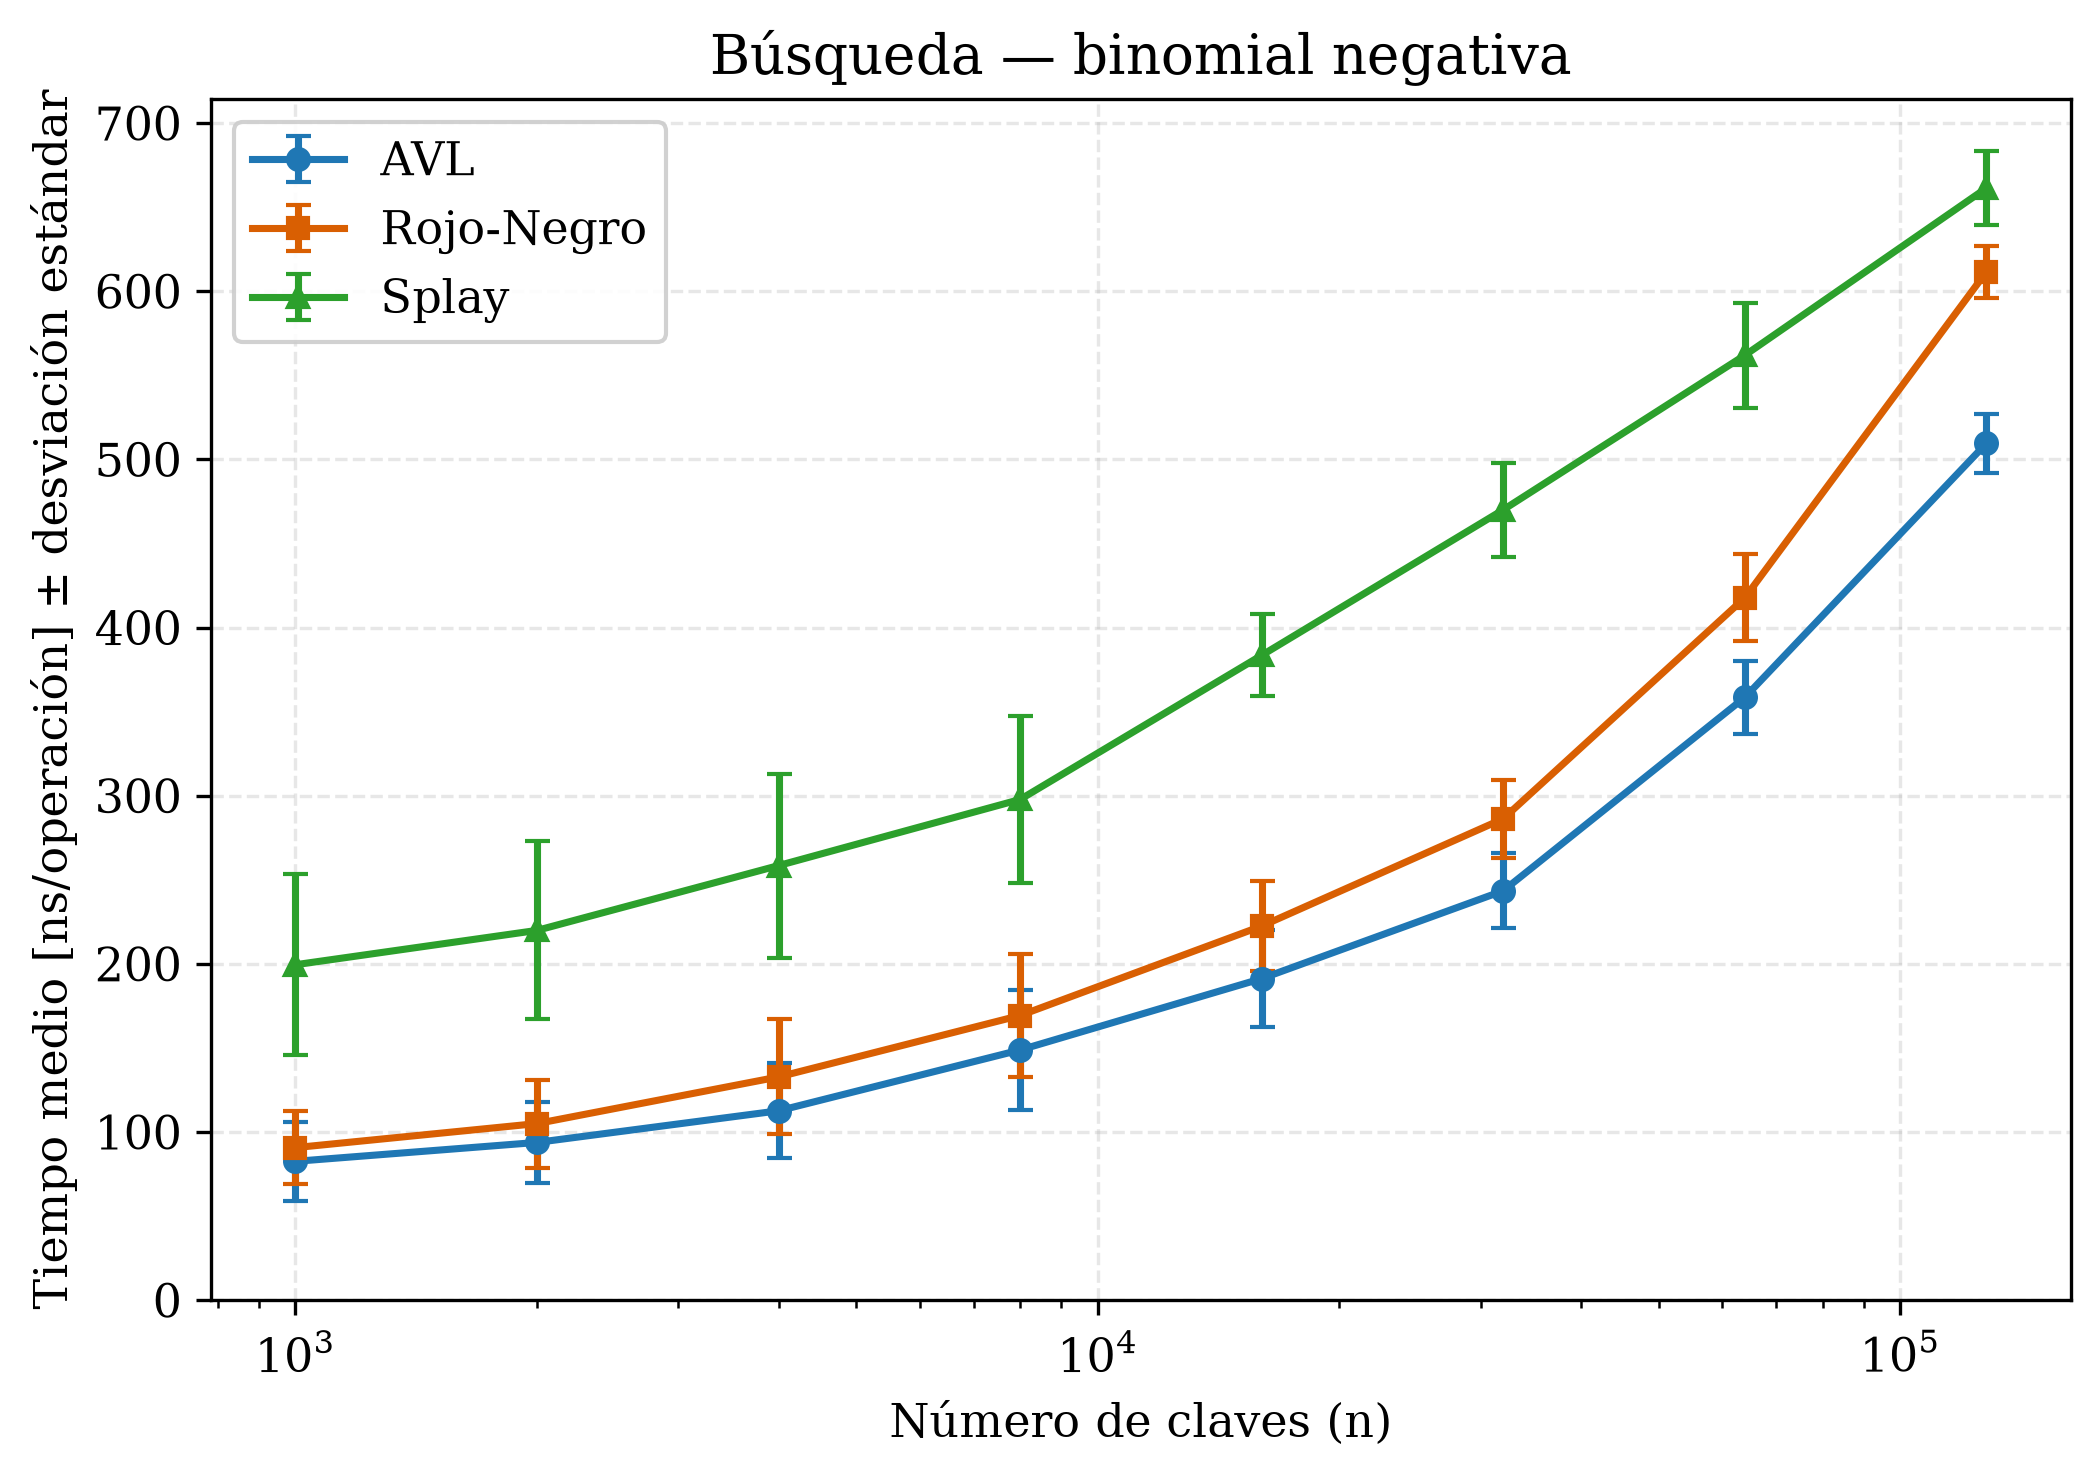
\includegraphics[width=\textwidth]{../plots/por_tamano/fig_busqueda_general_binomial_negativa.png}
        \caption{Consultas concentradas mediante binomial negativa.}
        \label{fig:b02-busqueda-binomial}
    \end{subfigure}
    \caption{Búsqueda: comparación entre árboles para cada patrón de acceso.
    Se cronometran $10n$ búsquedas después de $5n$ consultas de preparación.}
    \label{fig:b02-busquedas}
\end{figure}

\paragraph{Observaciones generales.}
La binomial negativa reduce la media de búsqueda respecto a la uniforme en
los tres árboles y en los ocho tamaños. En $n=128\,000$, AVL pasa de $606$ a
$509$ ns por búsqueda ($16\%$ menos), Rojo-Negro de $724$ a $611$ ns
($16\%$ menos) y Splay de $1\,352$ a $661$ ns ($51\%$ menos). La mejora
relativa de Splay es la mayor, como anticipaba la hipótesis, pero AVL conserva
el menor tiempo absoluto bajo ambas distribuciones en ese tamaño.

\begin{figure}[H]
    \centering
    \begin{subfigure}[t]{0.48\textwidth}
        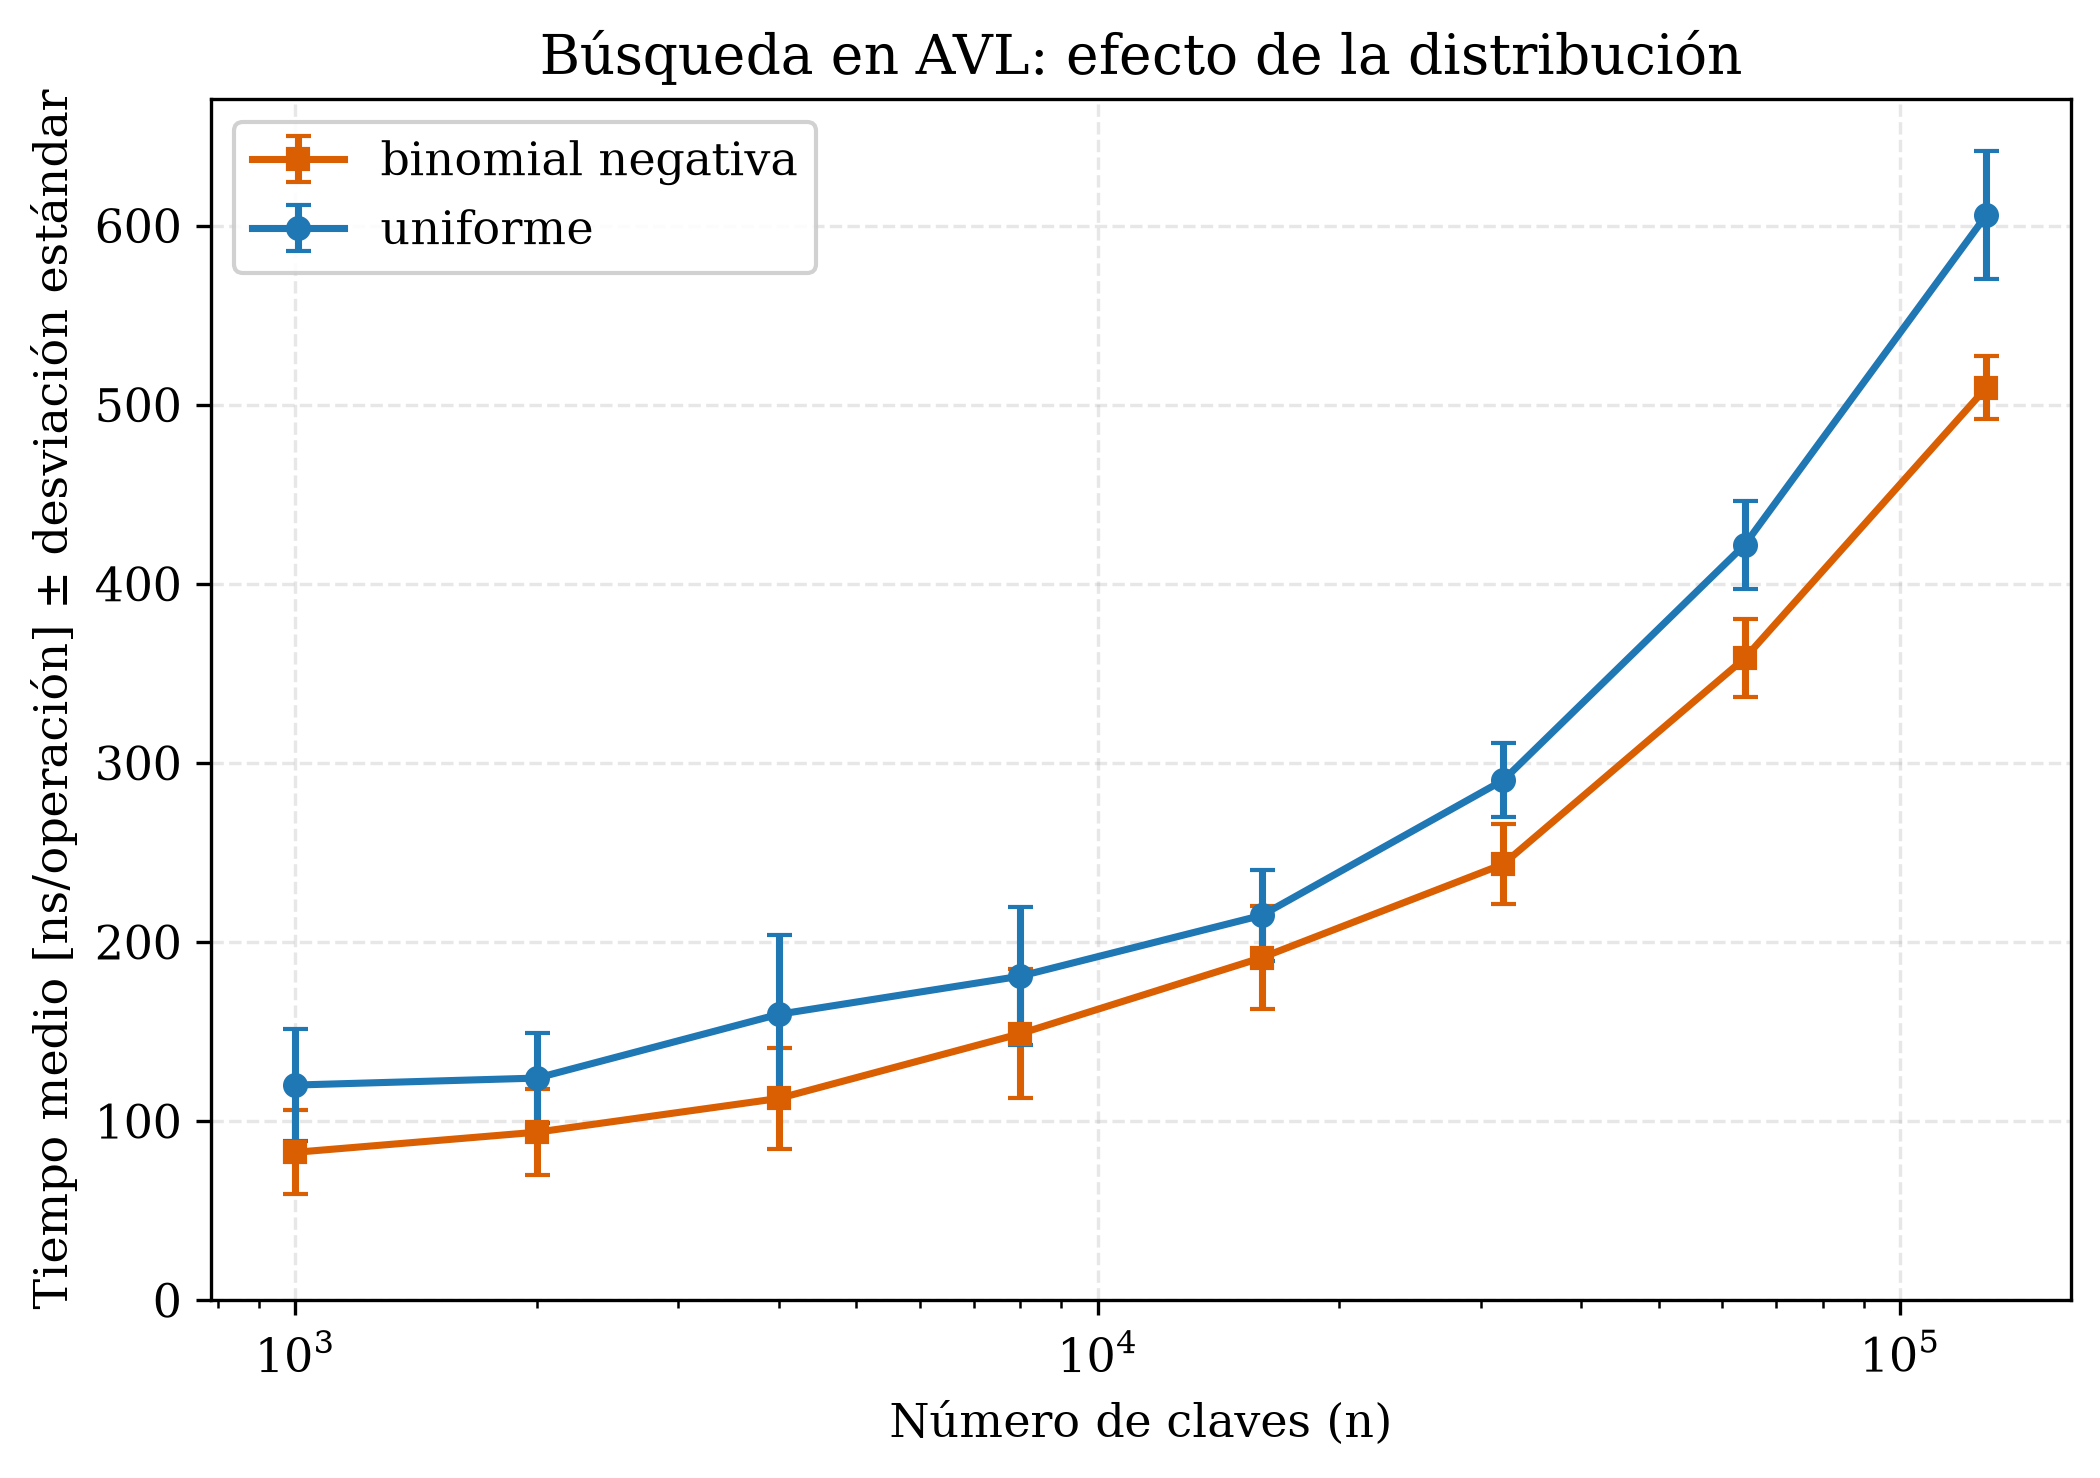
\includegraphics[width=\textwidth]{../plots/distribuciones/fig_distribuciones_avl.png}
        \caption{AVL: uniforme frente a binomial negativa.}
        \label{fig:b02-dist-avl}
    \end{subfigure}
    \hfill
    \begin{subfigure}[t]{0.48\textwidth}
        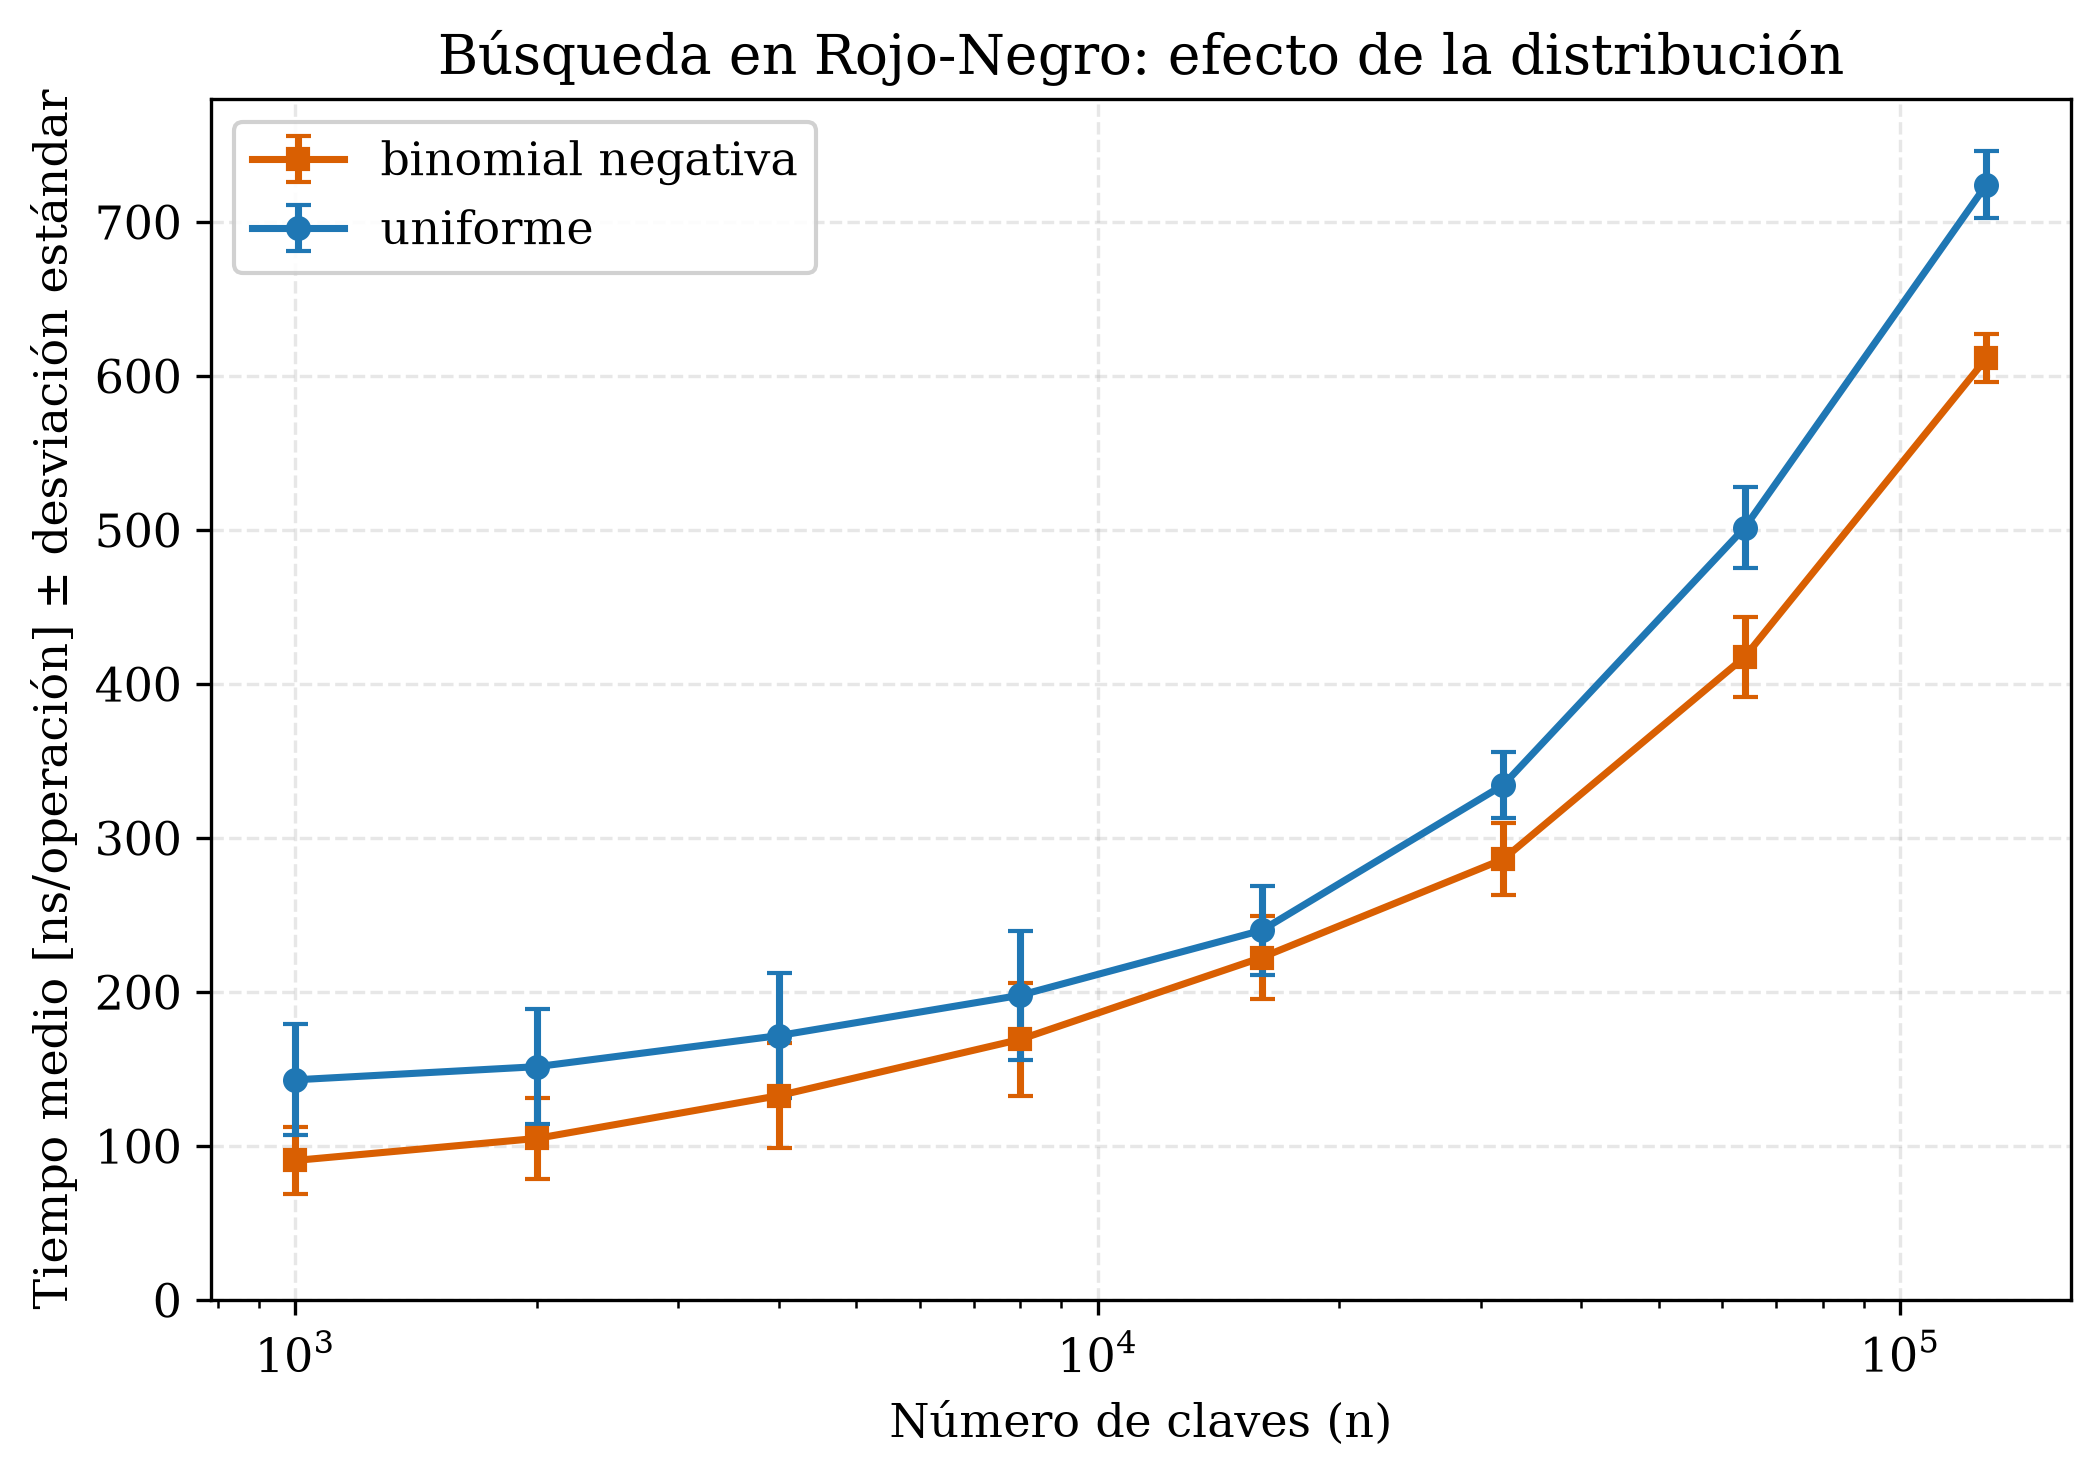
\includegraphics[width=\textwidth]{../plots/distribuciones/fig_distribuciones_rojo_negro.png}
        \caption{Rojo-Negro: las mismas dos cargas.}
        \label{fig:b02-dist-rb}
    \end{subfigure}
    \vskip\baselineskip
    \begin{subfigure}[t]{0.64\textwidth}
        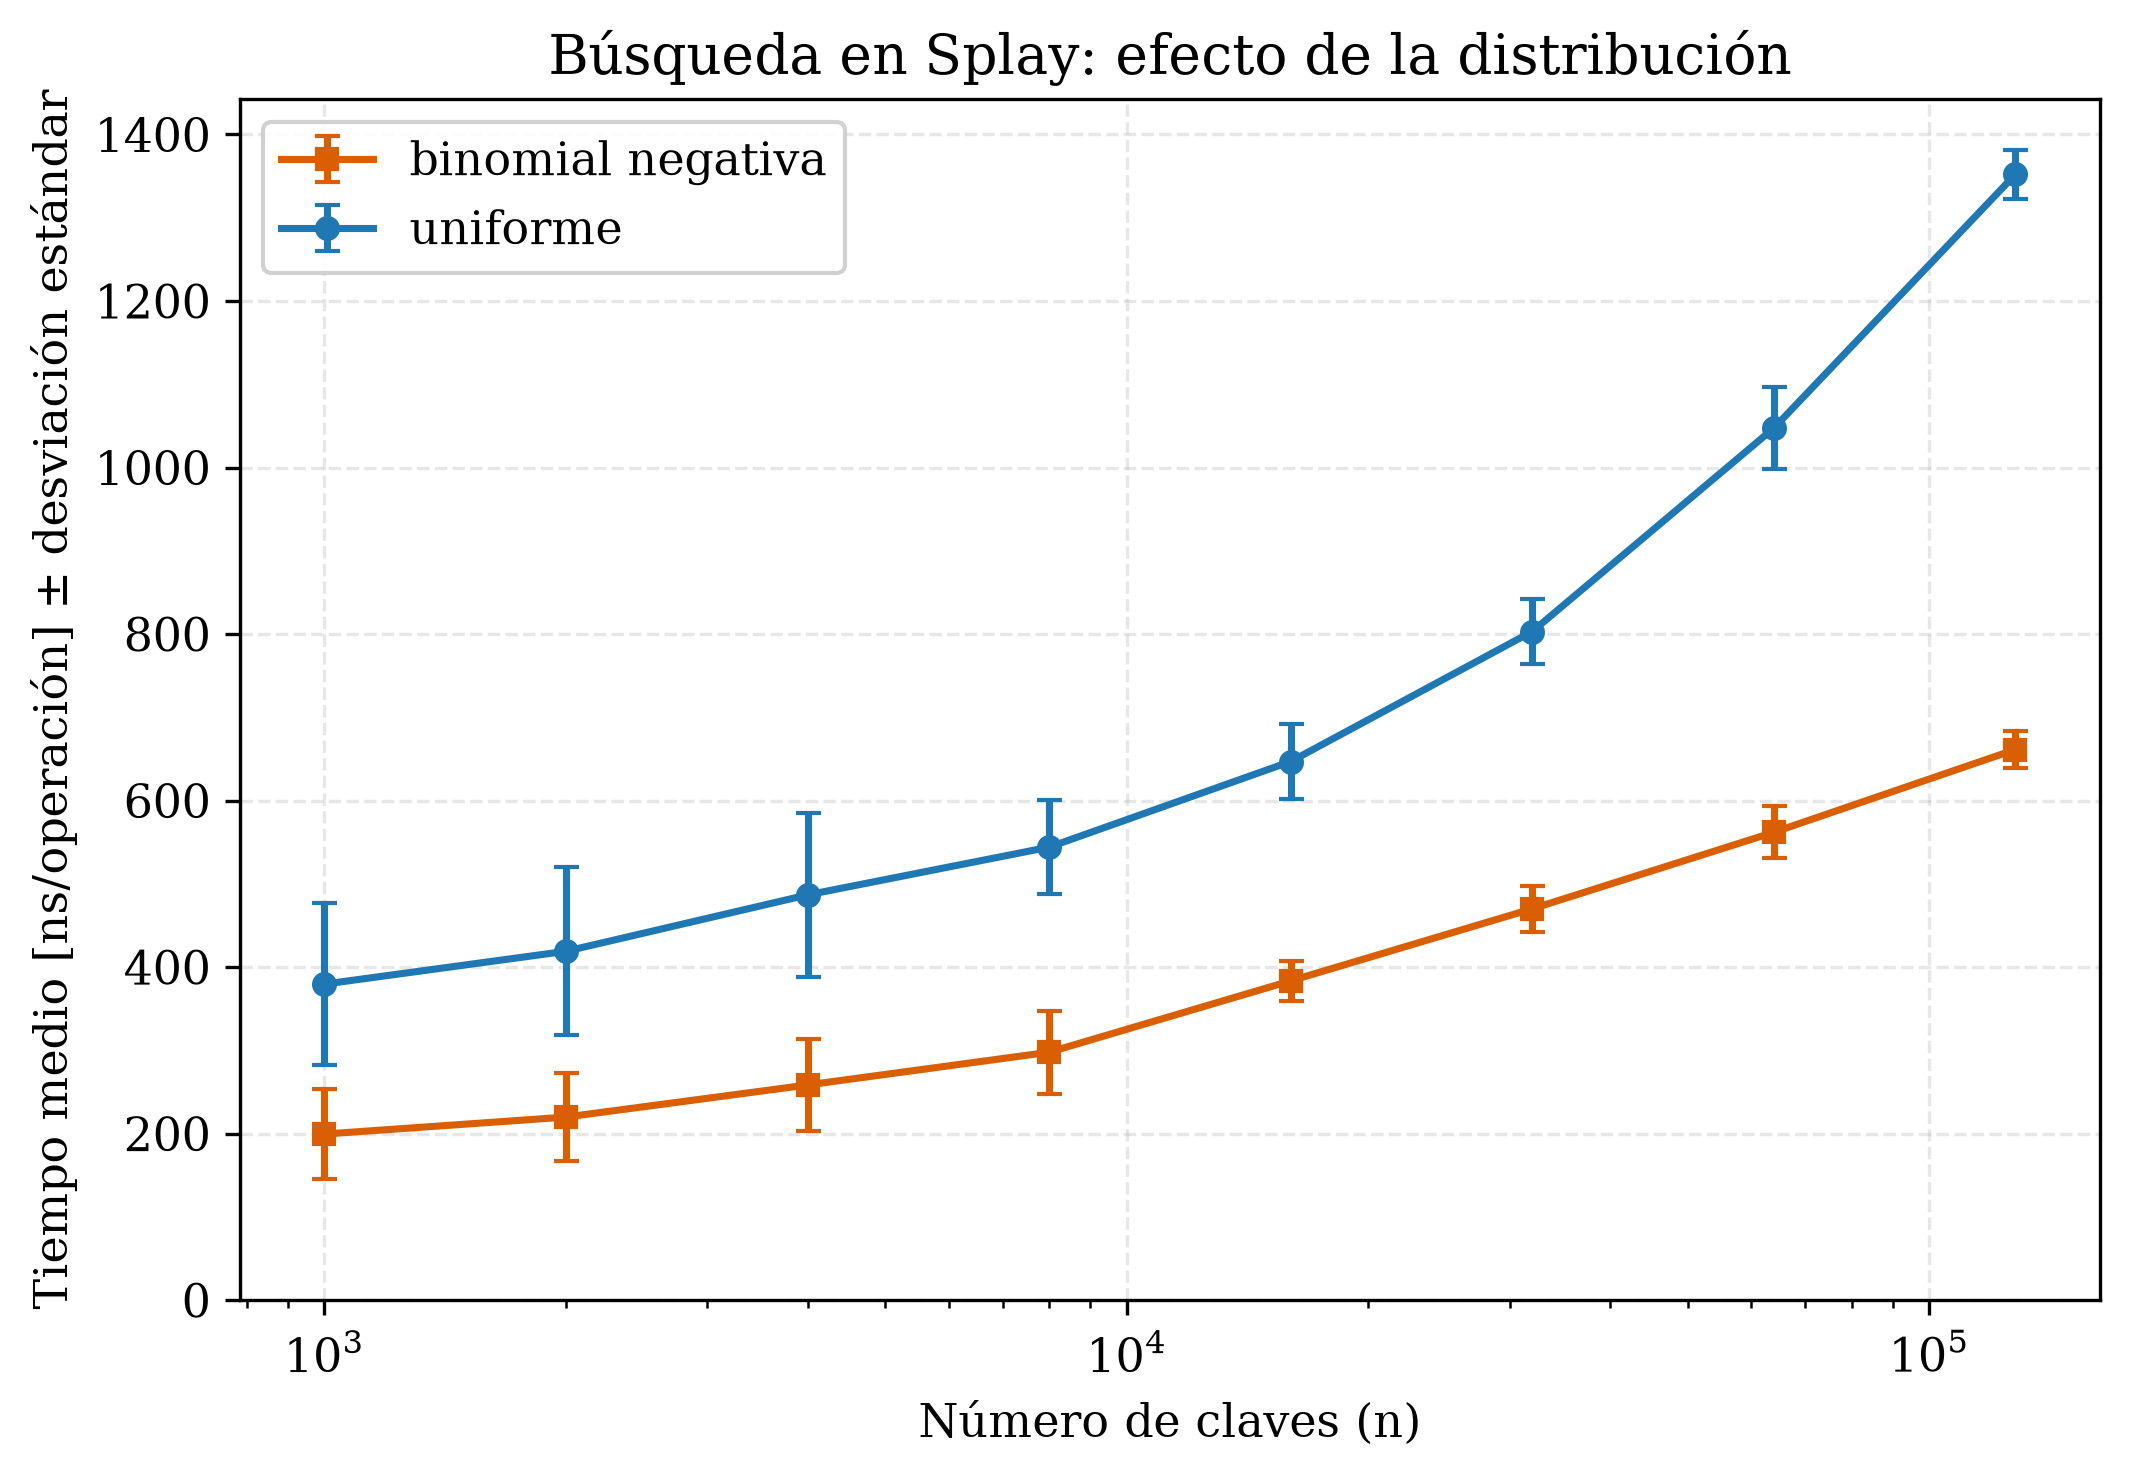
\includegraphics[width=\textwidth]{../plots/distribuciones/fig_distribuciones_splay.png}
        \caption{Splay: efecto de consultar repetidamente claves populares.}
        \label{fig:b02-dist-splay}
    \end{subfigure}
    \caption{Efecto de la distribución dentro de cada implementación.
    Cada par de curvas corresponde al mismo árbol y tamaño inicial $n$.}
    \label{fig:b02-distribuciones}
\end{figure}

\paragraph{Lectura del contraste por árbol.}
Las tres figuras de \texttt{distribuciones/} muestran las mismas diferencias
desde la perspectiva de cada implementación. Puesto que AVL y Rojo-Negro
también mejoran sin autoajustarse, la diferencia entre cargas no puede
atribuirse exclusivamente a las rotaciones de Splay.

\subsubsection{Experimento 3: Vaciado completo antes y después de consultas}

La Figura~\ref{fig:b02-d0} representa D0: se vacían los tres árboles sin
búsquedas previas y se mide el tiempo medio por una de las $n$ eliminaciones.
Las Figuras~\ref{fig:b02-d1-uniforme} y~\ref{fig:b02-d1-binomial}
representan D1: se vacía \emph{solo Splay} después de $15n$ búsquedas
uniformes o binomiales negativas, respectivamente. D1 mide únicamente las
eliminaciones; ninguna búsqueda previa entra en ese tiempo. Para un mismo
$n$ y repetición, los tres escenarios usan el mismo orden de eliminación.

\paragraph{Hipótesis.}
En D0 se espera que el árbol Rojo-Negro ofrezca un vaciado competitivo por
operación. En D1 se espera que el patrón de consultas previas pueda alterar
el costo posterior de vaciar Splay, puesto que cambia su forma. No existe una
garantía teórica de que concentrar las búsquedas acelere todas las
eliminaciones: durante el vaciado se retiran también claves poco consultadas
y la estructura vuelve a modificarse.

\begin{figure}[H]
    \centering
    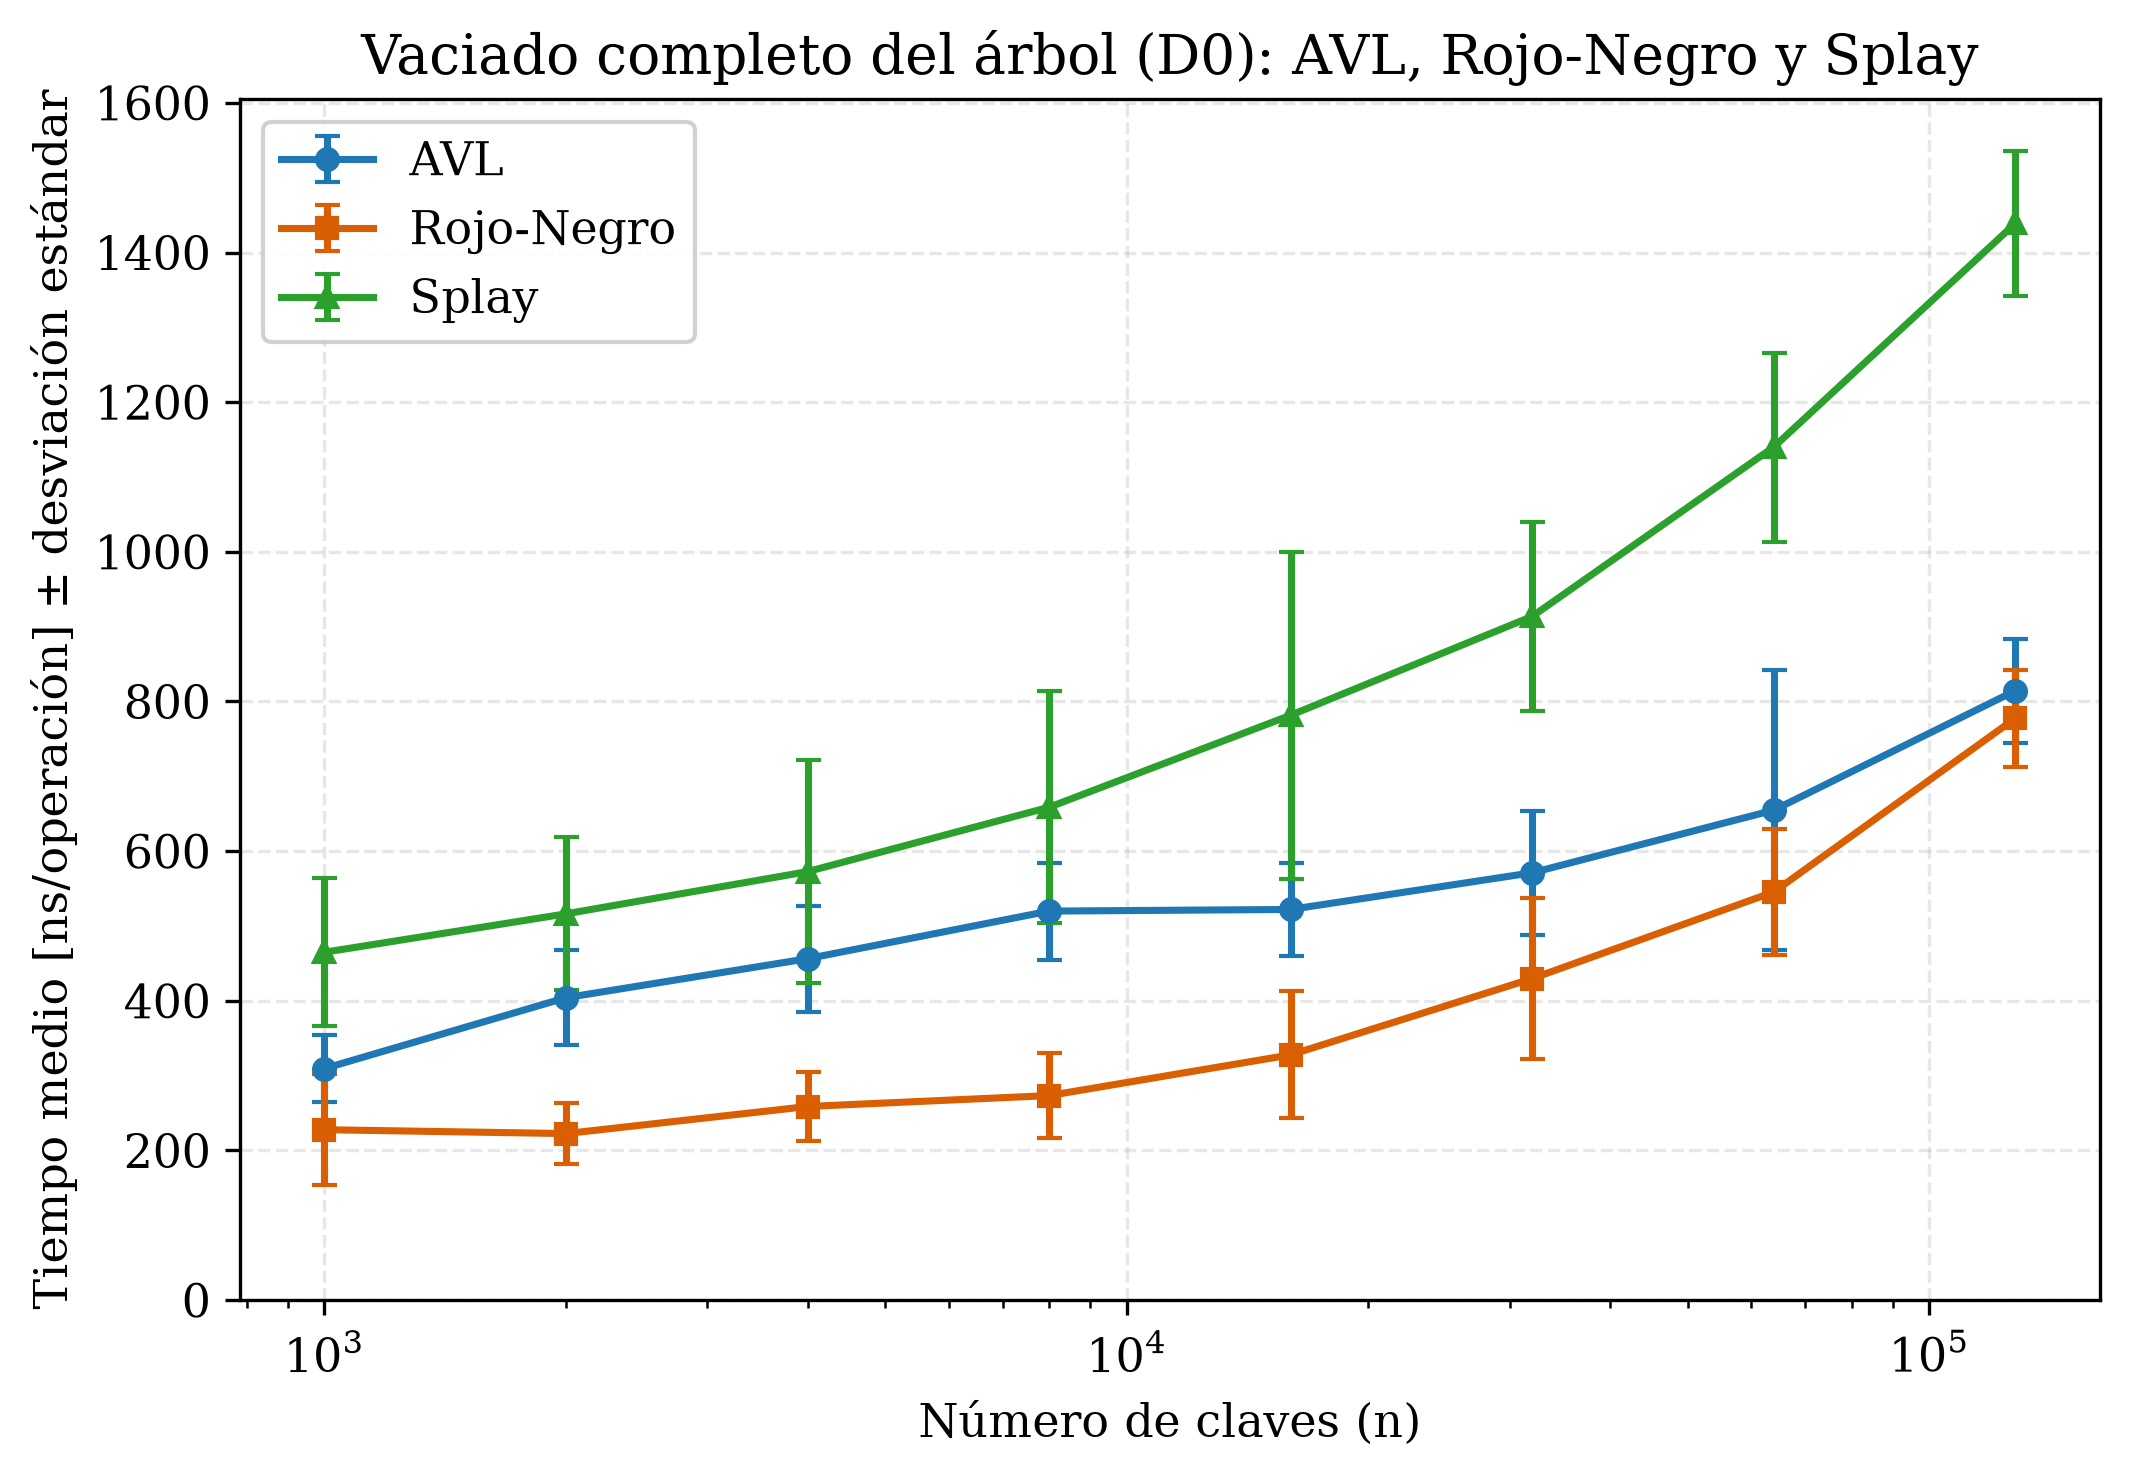
\includegraphics[width=0.84\textwidth]{../plots/por_tamano/fig_eliminacion_d0_sin_especificar.png}
    \caption{D0: vaciado completo sin consultas previas. Se comparan AVL,
    Rojo-Negro y Splay con las mismas claves y el mismo orden de eliminación.}
    \label{fig:b02-d0}
\end{figure}

\paragraph{Observación de D0.}
El Rojo-Negro obtiene el menor tiempo medio de vaciado en los ocho tamaños.
Para $n=128\,000$ registra $778$ ns por eliminación, frente a $814$ ns de
AVL y $1\,439$ ns de Splay.

\begin{figure}[H]
    \centering
    \begin{subfigure}[t]{0.48\textwidth}
        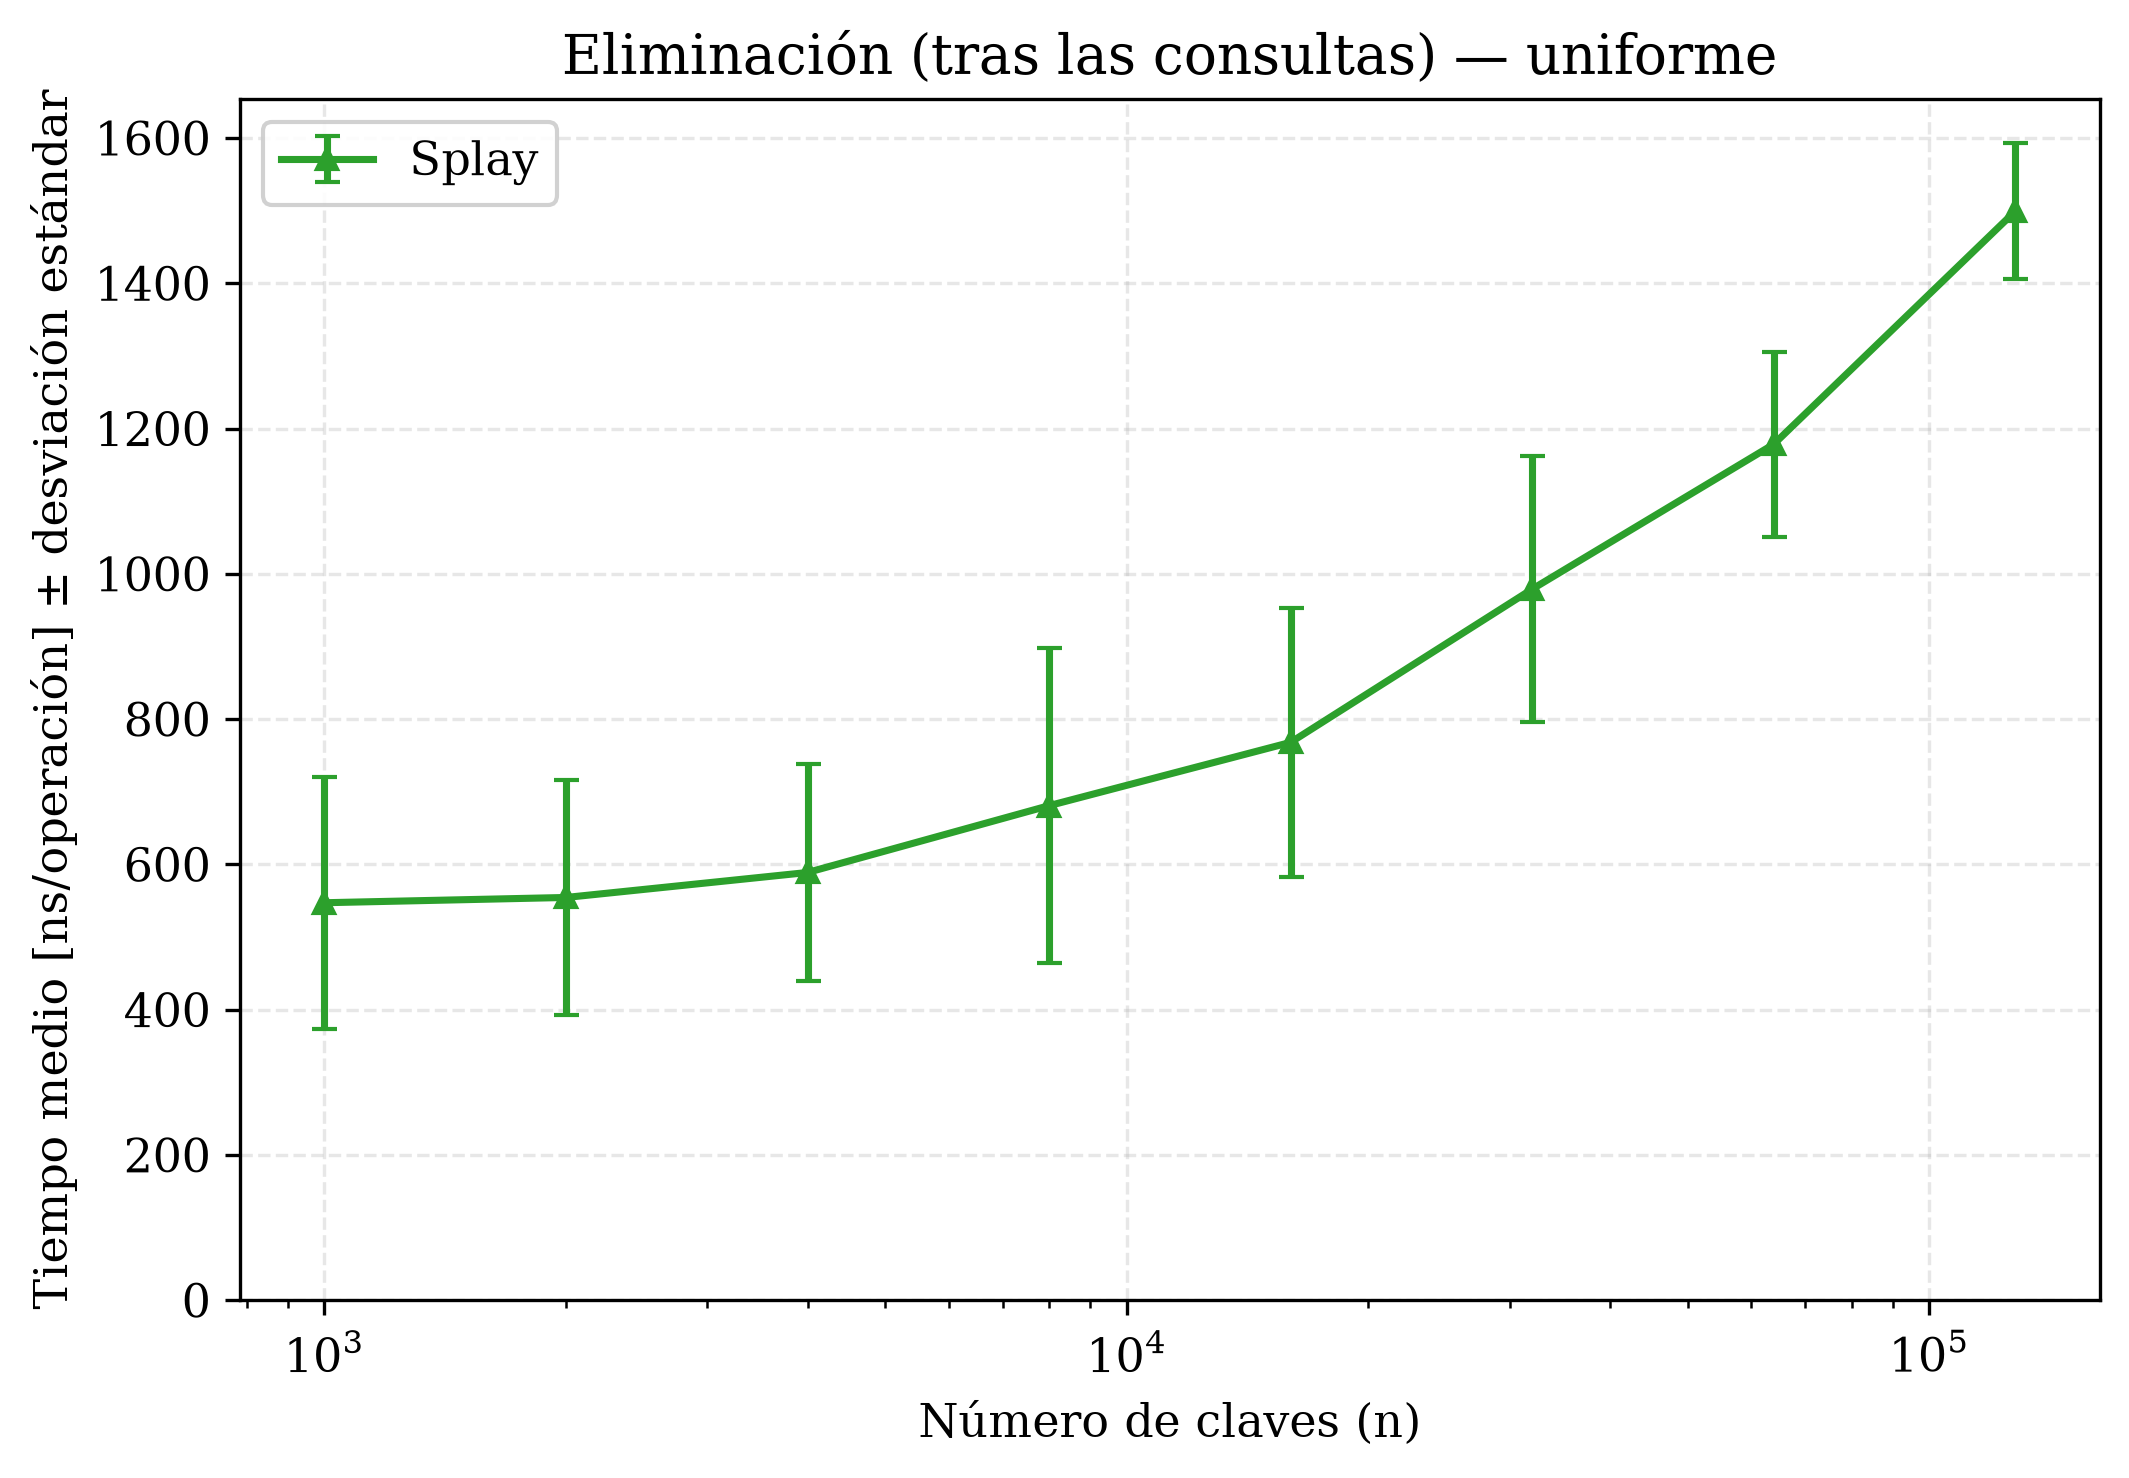
\includegraphics[width=\textwidth]{../plots/por_tamano/fig_eliminacion_d1_uniforme.png}
        \caption{Splay después de consultas uniformes.}
        \label{fig:b02-d1-uniforme}
    \end{subfigure}
    \hfill
    \begin{subfigure}[t]{0.48\textwidth}
        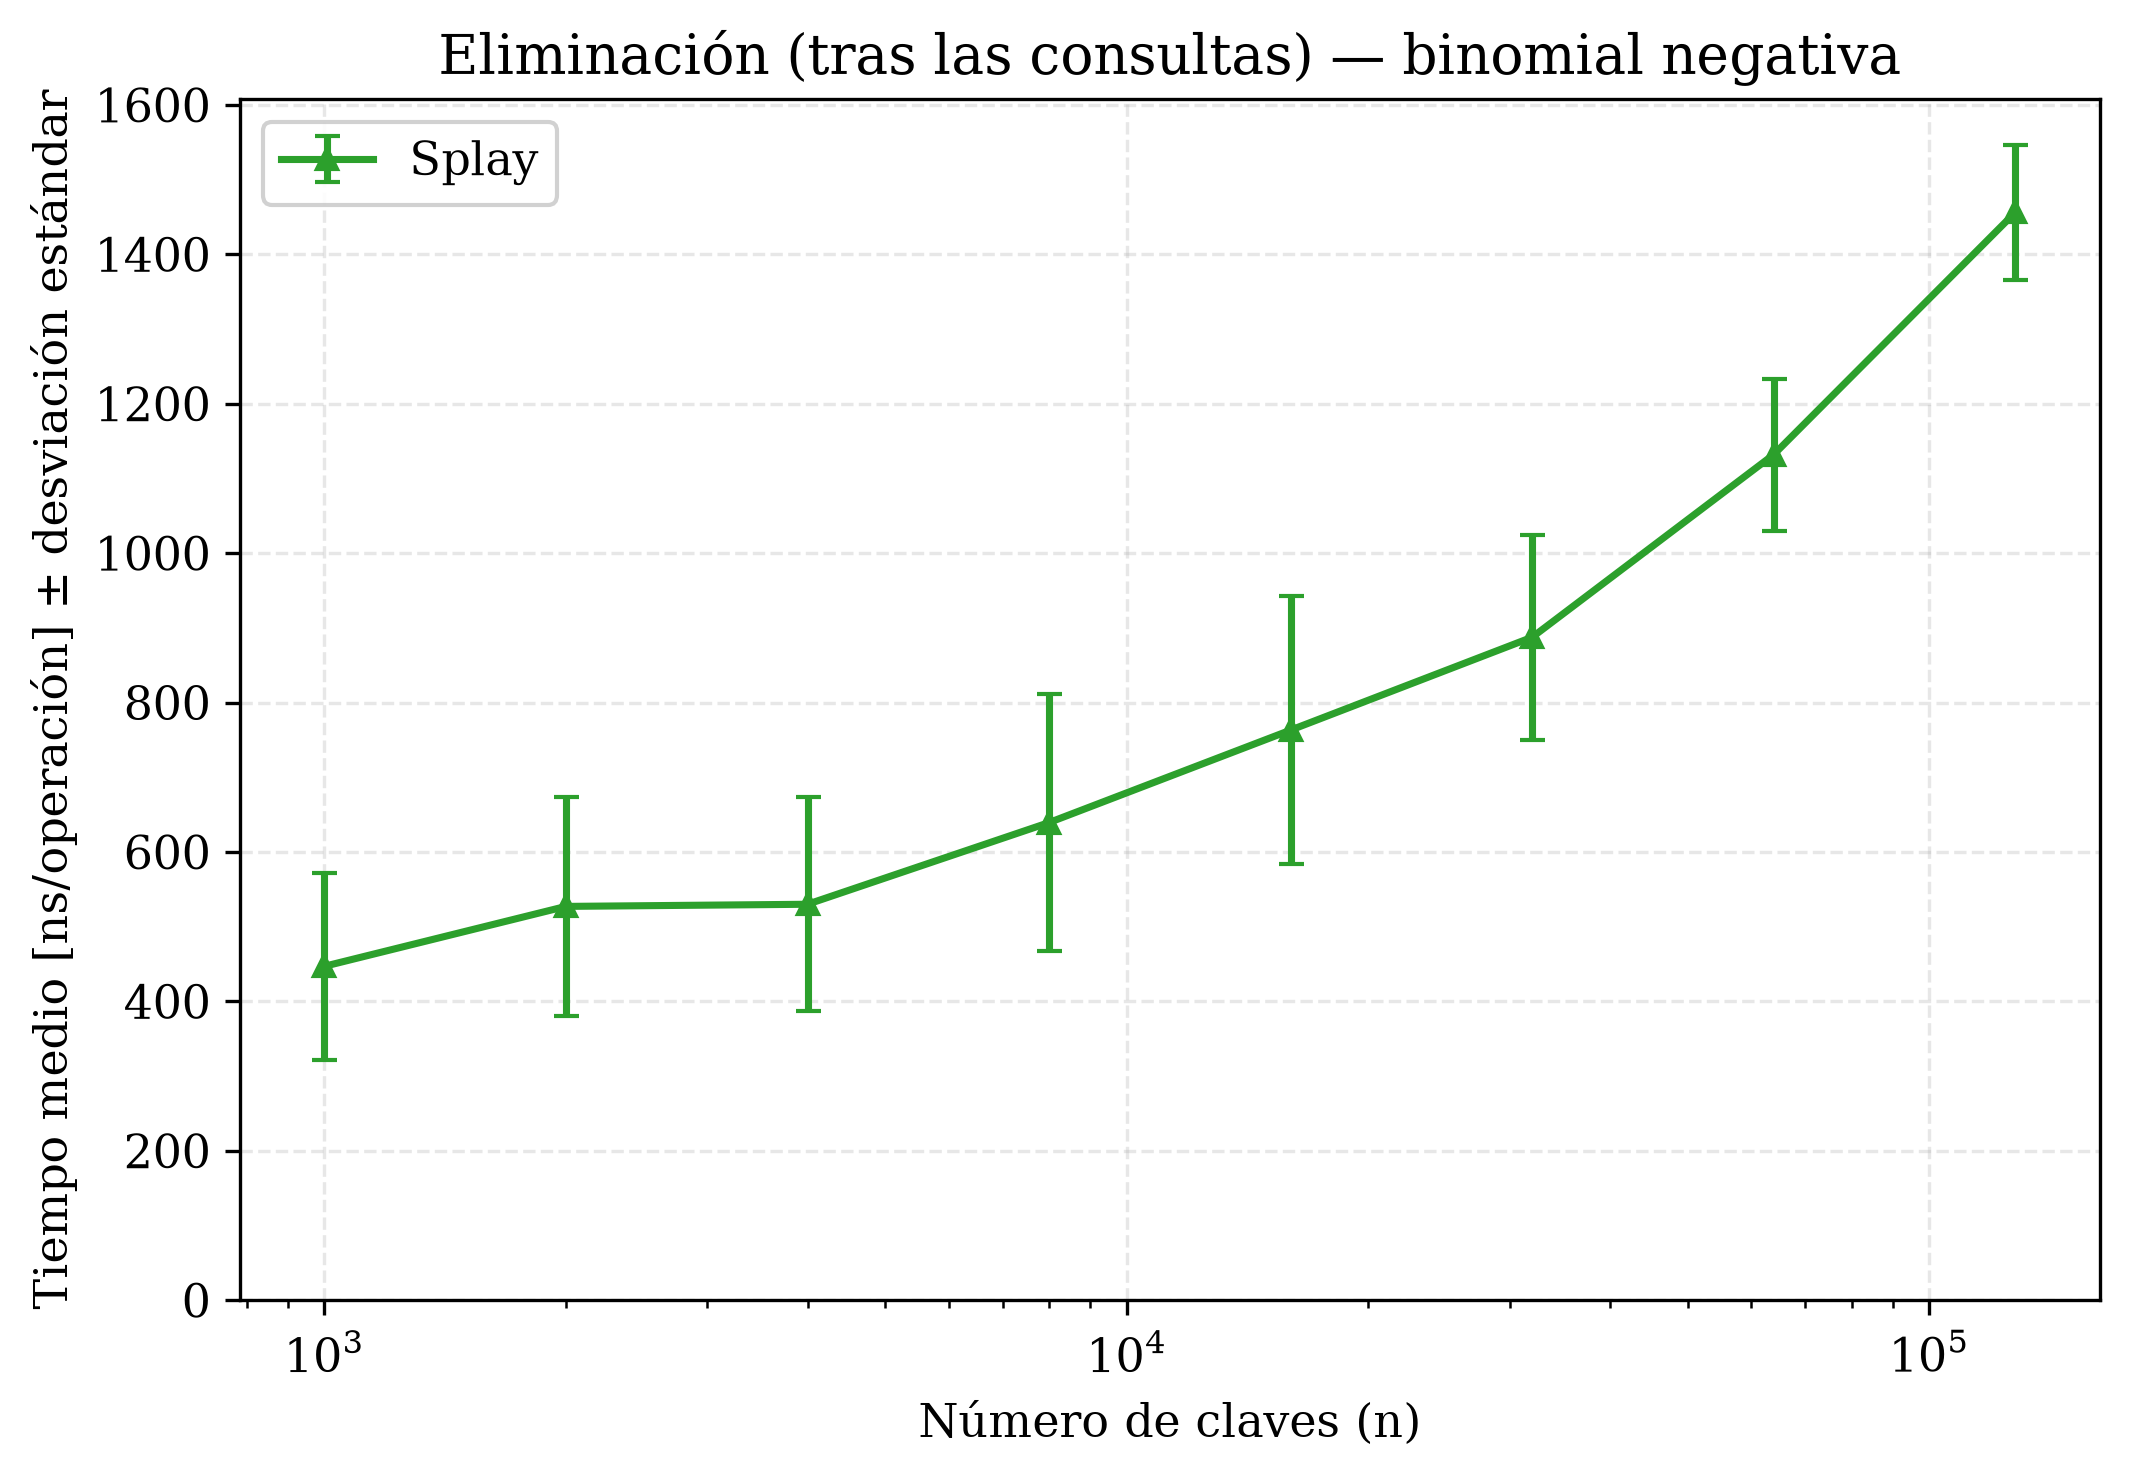
\includegraphics[width=\textwidth]{../plots/por_tamano/fig_eliminacion_d1_binomial_negativa.png}
        \caption{Splay después de consultas binomiales negativas.}
        \label{fig:b02-d1-binomial}
    \end{subfigure}
    \caption{D1: tiempo del vaciado de Splay condicionado por el patrón de
    consultas \emph{anterior} a la medición. En ambos casos, las $n$ claves se
    eliminan en el mismo orden; la distribución no determina qué se borra.}
    \label{fig:b02-d1}
\end{figure}

\paragraph{Observación de D1.}
La media de Splay tras binomial negativa es
menor que tras uniforme en los ocho tamaños; para $n=128\,000$ son $1\,456$
y $1\,499$ ns, respectivamente. Esa diferencia de $43$ ns (cerca de $3\%$)
es menor que las desviaciones estándar de ambas series, de unos $90$ ns, por
lo que no se puede afirmar un efecto concluyente solo con estas barras. El
D0 de Splay en ese tamaño fue $1\,439$ ns: las tres medias de vaciado están
próximas. Las búsquedas previas también pueden cambiar el estado de caché;
el diseño no separa ese efecto del cambio de forma del árbol.

\newpage
\section{Conclusiones}


Los tres árboles ofrecen propiedades teóricas distintas, pero la selección
práctica depende también de la operación y del patrón de acceso. Los resultados experimentales
permite extraer las siguientes conclusiones para estas implementaciones y los tamaños $1\,000\leq n\leq128\,000$:

\begin{enumerate}
    \item \textbf{Inserción.} El adaptador Rojo-Negro basado en
    \texttt{std::set} registró el menor tiempo medio en los ocho tamaños.
    Para $n=128\,000$ necesitó $470$ ns por clave, frente a $848$ ns de AVL
    y $1\,048$ ns de Splay. Esto debido a que el Rojo-Negro
    admite un balance menos estricto que AVL, cuyo código actualiza alturas
    y comprueba el equilibrio al regresar por el camino de inserción. También
    interviene la implementación optimizada de \texttt{std::set}; los tiempos
    por sí solos no permiten separar ambos efectos ni contar rotaciones.
    Splay, en cambio, lleva \emph{cada nueva clave} a la raíz mediante
    rotaciones y actualizaciones de punteros. Como el orden insertado está
    barajado y contiene claves únicas, ese trabajo adicional no explota
    todavía una localidad de accesos repetidos. Esto ofrece una explicación
    del mayor tiempo observado sin contradecir su costo amortizado
    $O(\log n)$ por operación.

    \item \textbf{Búsqueda uniforme.} AVL fue el más rápido en los ocho
    tamaños; en $n=128\,000$ registró $606$ ns por búsqueda, seguido por
    Rojo-Negro con $724$ ns y Splay con $1\,352$ ns. AVL y Rojo-Negro
    mantienen alturas acotadas y realizan la búsqueda sin modificar el
    árbol. Splay también posee una cota \emph{amortizada} $O(\log n)$,
    aunque una operación individual puede costar $O(n)$; no corresponde
    describir toda su curva como lineal por ese peor caso individual. Bajo
    consultas uniformes, llevar cada clave encontrada a la raíz introduce
    rotaciones cuya inversión rara vez favorece de forma persistente a un
    subconjunto pequeño. La combinación de recorridos y reajustes es
    compatible con su mayor tiempo medido.

    \item \textbf{Búsqueda con binomial negativa.} Concentrar las consultas
    mejoró las medias de los tres árboles, pero Splay mostró el mayor cambio
    relativo. En $n=128\,000$ pasó de $1\,352$ a $661$ ns por búsqueda,
    una reducción del $51\%$; AVL y Rojo-Negro mejoraron aproximadamente un
    $16\%$ cada uno. La repetición de claves populares permite que Splay
    las acerque a la raíz y reduzca recorridos posteriores. Esto no vuelve
    constante toda búsqueda: también se consultan otras claves y cada
    reajuste modifica los caminos siguientes. Dentro del rango ensayado, el
    tiempo de Splay bajo esta distribución creció por un factor de $3{,}3$
    entre los tamaños extremos, frente a $6{,}2$ en AVL y $6{,}7$ en
    Rojo-Negro; esos factores describen las curvas observadas, no una nueva
    cota asintótica. AVL y Rojo-Negro no se reestructuran al buscar, pero un
    conjunto consultado con frecuencia puede mejorar la localidad de caché
    y tener profundidades particulares en cada árbol. El experimento no
    separa esos mecanismos. Pese a la gran mejora relativa, AVL conservó el
    menor tiempo absoluto de búsqueda bajo binomial negativa.

La concentración de consultas benefició la búsqueda de los tres árboles,
con el mayor cambio proporcional en Splay: a $n=128\,000$ su media se redujo
aproximadamente a la mitad frente a consultas uniformes. Sin embargo, ese
beneficio no le dio el menor tiempo absoluto de búsqueda. El patrón previo
de consultas produjo diferencias menores en el vaciado de Splay. Como las
figuras presentan desviaciones estándar y no una prueba de significancia,
no se atribuye causalmente esa pequeña diferencia a una reestructuración
ventajosa.
    \item \textbf{Eliminación y efecto de las consultas previas.} En el
    vaciado D0, Rojo-Negro registró la menor media en todos los tamaños. En
    $n=128\,000$ obtuvo $778$ ns por clave, cercano a los $814$ ns de AVL
    y por debajo de los $1\,439$ ns de Splay. El balance menos estricto de
    Rojo-Negro puede reducir parte del mantenimiento, pero la diferencia
    entre esas dos implementaciones también depende de su código y no se
    puede atribuir únicamente al número de rebalanceos. La eliminación de
    Splay busca y lleva la clave a la raíz; además, cuando existe un
    subárbol izquierdo, reajusta su máximo antes de unir los subárboles.
    Ese trabajo es compatible con su mayor constante temporal, aun cuando
    una secuencia de eliminaciones conserva costo amortizado logarítmico.

    En D1 se vacía Splay después de las consultas, siempre con el mismo
    orden de eliminación. A $n=128\,000$, las medias fueron $1\,499$ ns
    tras consultas uniformes y $1\,456$ ns tras binomial negativa, frente a
    $1\,439$ ns en D0. La ventaja de búsqueda bajo sesgo apenas se traslada
    al vaciado: se elimina \emph{cada} clave una vez y el propio proceso
    modifica continuamente el árbol, de modo que la cercanía inicial de
    las claves populares pierde relevancia. Esta es una interpretación
    plausible, no una causa demostrada. La diferencia de $43$ ns entre los
    dos D1 es menor que sus desviaciones estándar, cercanas a $90$ ns; las
    consultas previas también afectan la caché. Con los resúmenes actuales
    no hay evidencia suficiente para afirmar una mejora concluyente del
    tiempo de eliminación por la distribución de consultas.
\end{enumerate}

En conjunto, \texttt{std::set} fue la opción más rápida para insertar y
vaciar en esta experimentación, mientras que AVL ofreció la menor latencia de
búsqueda en ambas cargas. Splay aprovechó especialmente la repetición de
claves en términos relativos, pero no superó a AVL en tiempo absoluto.
Estas conclusiones se limitan al entorno, implementaciones y cargas
medidos; no establecen una jerarquía universal entre los tres árboles.

\newpage
\section{Referencias}



\begingroup
\renewcommand{\section}[2]{}% Suprime titulo duplicado generado internamente por thebibliography
\begin{thebibliography}{9}

\bibitem{adelson1962}
G. M. Adelson-Vel'skii y E. M. Landis,
``An algorithm for the organization of information,''
\textit{Doklady Akademii Nauk SSSR}, vol. 146, n.º 2, pp. 263--266, 1962.
Disponible en:
\url{https://www.mathnet.ru/php/archive.phtml?jrnid=dan&option_lang=eng&paperid=26964&wshow=paper}.

\bibitem{avlNotes}
R. W. Holte,
``Height-Balanced Binary Search Trees,''
University of Alberta, notas de curso.
Disponible en:
\url{https://webdocs.cs.ualberta.ca/~holte/T26/avl-trees.html}.

\bibitem{cppAssociative}
ISO C++ working draft,
``Associative containers.''
Requisitos de complejidad para búsqueda, inserción y eliminación en
contenedores asociativos.
Disponible en:
\url{https://eel.is/c++draft/associative}.

\bibitem{splay1985}
D. D. Sleator y R. E. Tarjan,
``Self-Adjusting Binary Search Trees,''
\textit{Journal of the ACM}, vol. 32, n.º 3, pp. 652--686, 1985.
Disponible en:
\url{https://www.cs.cmu.edu/~sleator/papers/Self-Adjusting.htm}.


\bibitem{agarwalAgAVLTree}
A. Agarwal,
\textit{AgAVLTree: C++ AVL Tree Implementation}.
Repositorio GitHub; licencia MIT.
\url{https://github.com/Aditya-A-garwal/AgAVLTree/blob/main/src/AgAVLTree.h}

\bibitem{boostSplay}
Boost C++ Libraries,
\textit{Boost.Intrusive: splaytree\_algorithms.hpp}.
Repositorio GitHub; licencia Boost Software License 1.0.
\url{https://github.com/boostorg/intrusive/blob/develop/include/boost/intrusive/splaytree_algorithms.hpp}

\bibitem{gccSet}
GCC Project,
\textit{GNU libstdc++: stl\_set.h}.
Repositorio GitHub.
\url{https://github.com/gcc-mirror/gcc/blob/master/libstdc++-v3/include/bits/stl_set.h}

\bibitem{gccTree}
GCC Project,
\textit{GNU libstdc++: stl\_tree.h}.
Repositorio GitHub.
\url{https://github.com/gcc-mirror/gcc/blob/master/libstdc++-v3/include/bits/stl_tree.h}

\bibitem{agarwal_agavltree}
A. Agarwal,
\textit{AgAVLTree.h},
código fuente, AgAVLTree.
\url{https://github.com/Aditya-A-garwal/AgAVLTree/blob/main/src/AgAVLTree.h}.

\bibitem{gaztanaga_splaytree}
I. Gaztanaga,
\textit{splaytree\_algorithms.hpp},
código fuente, Boost.Intrusive.
\url{https://github.com/boostorg/intrusive/blob/develop/include/boost/intrusive/splaytree_algorithms.hpp}.

\end{thebibliography}

\subsection{Usos Específicos}

El código fuente desarrollado, los scripts de automatización del banco de pruebas y los datasets generados para este boletín se encuentran alojados en el repositorio de reproducibilidad del proyecto: \url{https://github.com/StackDs/EDAA-Experiments}.


\subsection{Declaración De Uso De IA Generativa}
Durante la elaboración de este informe se utilizó ChatGPT, de OpenAI,
como herramienta de apoyo para revisar la redacción académica,
discutir el análisis de complejidad de los algoritmos y contrastar
dicho análisis con las implementaciones estudiadas.
De igual forma se utilizó Google Gemini para estructurar el repositorio con el código fuente y para mejorar los experimentos en términos de optimización.
La responsabilidad por el contenido final, la interpretación de
los resultados y la exactitud de las referencias corresponde
al autor del informe.


\end{document}
